\documentclass[11pt,a4paper,oneside]{article}
\usepackage[margin=2.35cm,top=2.4cm,bottom=2.45cm,headheight=16pt]{geometry}
\usepackage{fontspec}
\usepackage{polyglossia}
\setmainlanguage{spanish}
\setmainfont{Noto Serif}
\setsansfont{DejaVu Sans}
\setmonofont{Noto Sans Mono}[Scale=0.83]
\usepackage{amsmath,amssymb,mathtools}
\usepackage{graphicx,xcolor,booktabs,longtable,array,tabularx,calc}
\usepackage{microtype,enumitem,fancyhdr,titlesec,caption,float}
\usepackage{hyperref}
\usepackage{minted}
\usepackage{newunicodechar}
\newunicodechar{✓}{{\fontspec{DejaVu Sans}✓}}
\definecolor{navy}{HTML}{142C40}
\definecolor{teal}{HTML}{087E83}
\definecolor{ochre}{HTML}{A76439}
\definecolor{codebg}{HTML}{F2F6F6}
\hypersetup{colorlinks=true,linkcolor=teal,urlcolor=teal,citecolor=teal,
 pdfauthor={Jhasbleidy Rodríguez Cárdenas; Sebastián Palacio},pdftitle={Cuando un radionúclido decae dentro del ADN humano}}
\setlength{\parindent}{0pt}
\setlength{\parskip}{5pt plus 1pt}
\emergencystretch=3em
\providecommand{\tightlist}{\setlength{\itemsep}{0pt}\setlength{\parskip}{0pt}}
\setlength{\tabcolsep}{4pt}
\renewcommand{\arraystretch}{1.17}
\titleformat{\section}{\sffamily\Large\bfseries\color{navy}}{\thesection}{.7em}{}
\titleformat{\subsection}{\sffamily\normalsize\bfseries\color{teal}}{\thesubsection}{.65em}{}
\titleformat{\subsubsection}{\sffamily\normalsize\bfseries\color{navy}}{\thesubsubsection}{.65em}{}
\titlespacing*{\section}{0pt}{21pt}{9pt}
\titlespacing*{\subsection}{0pt}{15pt}{6pt}
\captionsetup{font=small,labelfont={bf,color=teal},skip=6pt}
\renewcommand{\figurename}{Figura}
\renewcommand{\contentsname}{Índice general}
\renewcommand{\listfigurename}{Lista de figuras}
\setcounter{tocdepth}{2}
\setcounter{secnumdepth}{3}
\setkeys{Gin}{width=.94\linewidth,height=.31\textheight,keepaspectratio}
\pagestyle{fancy}
\fancyhf{}
\fancyhead[L]{\sffamily\footnotesize\color{teal} RADIOGENOMA · FÍSICA SUBATÓMICA}
\fancyhead[R]{\sffamily\footnotesize\color{navy} ADN HUMANO}
\fancyfoot[C]{\sffamily\footnotesize\color{navy}\thepage}
\renewcommand{\headrulewidth}{.4pt}
\setminted{fontsize=\footnotesize,breaklines,breakanywhere,linenos,numbersep=5pt,
 tabsize=2,frame=lines,framesep=2mm,bgcolor=codebg,baselinestretch=1.0}
\begin{document}
\begin{titlepage}
\thispagestyle{empty}
\color{navy}
\vspace*{1cm}
{\sffamily\large\bfseries UNIVERSIDAD NACIONAL DE COLOMBIA\par}
{\sffamily Departamento de Física · Física Subatómica\par}
\vspace{1.6cm}
{\sffamily\Huge\bfseries Cuando un radionúclido decae dentro del ADN humano\par}
\vspace{.5cm}
{\sffamily\Large\color{teal} Versión T · desarrollo teórico y computacional\par}
\vspace{.8cm}
\color{teal}\rule{\linewidth}{1.4pt}\color{navy}
\vspace{.5cm}
\begin{center}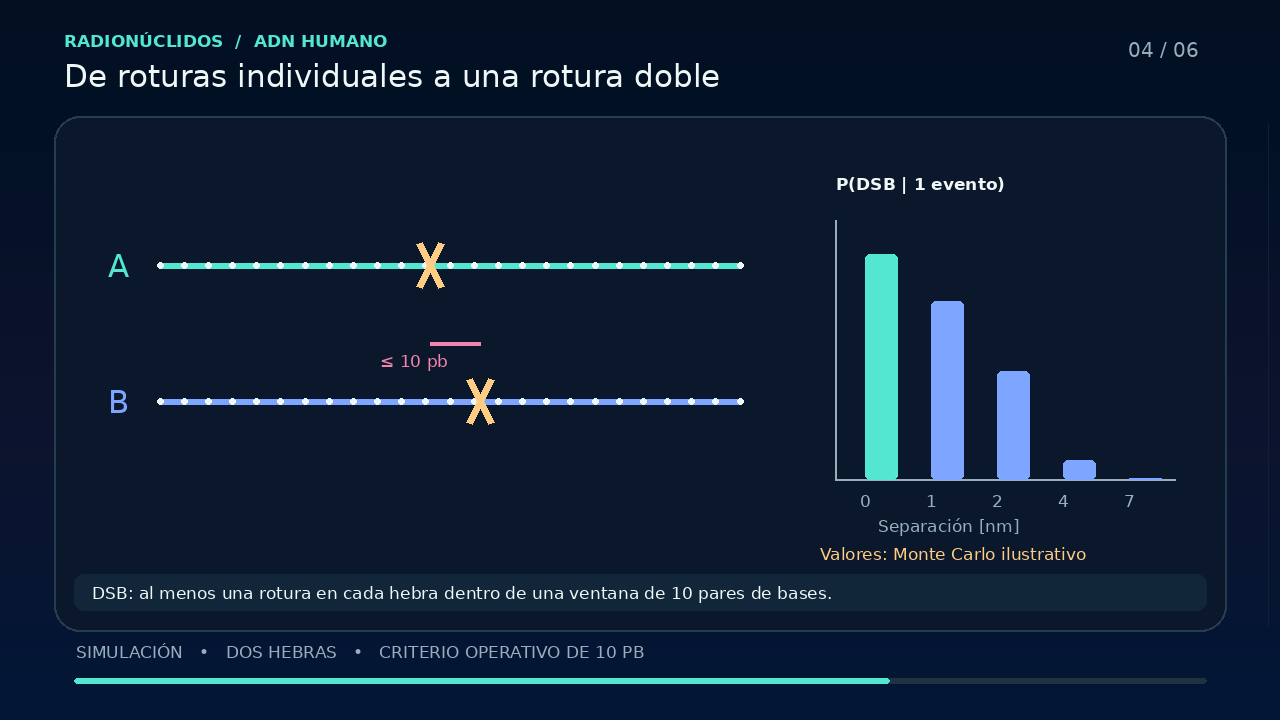
\includegraphics[width=.88\textwidth]{../media/04_roturas_agrupadas_portada.png}\end{center}
\vfill
{\sffamily\large Proyecto RadioGenoma\par}
{\sffamily Jhasbleidy Rodríguez Cárdenas · Sebastián Palacio\par}
{\sffamily Profesor: Jhon Morales Aponte\par}
{\sffamily Bogotá, Colombia · 25 de noviembre de 2026\par}
\vspace{.5cm}
{\small Artículo conductor: Whaley y Little (1990). Figuras y simulaciones propias;
las estimaciones del modelo se distinguen de datos publicados.\par}
\end{titlepage}
\pagenumbering{roman}
\begingroup\footnotesize\tableofcontents\endgroup
\clearpage
\listoffigures
\clearpage
\pagenumbering{arabic}
\section*{Resumen}\addcontentsline{toc}{section}{Resumen}

Esta monografía reconstruye una cadena causal desde la captura electrónica de \(^{125}\)I y el decaimiento beta menos de \(^{131}\)I hasta los efectos celulares observables cuando estos radionúclidos se incorporan a iododesoxiuridina. El experimento de Whaley y Little {[}1{]} comparó dos líneas linfoblastoides humanas con diferente capacidad de incorporar el análogo al ADN, TK6 y SE30, y cuantificó supervivencia y mutantes del locus \emph{hprt}. Se deriva la ley exponencial y un modelo de dos riesgos competitivos para distinguir semivida de residencia celular. Una geometría idealizada de 60 pares de bases permite definir distancias tridimensionales, probabilidades fenomenológicas de rotura y un criterio operacional de rotura doble. Se implementan simulaciones Monte Carlo con semilla fija, error estándar, control analítico, sensibilidad de parámetros y pruebas automatizadas. Las ecuaciones de reparación y mutación representan estados competidores con tasas declaradamente hipotéticas. La única pendiente experimental de mutantes utilizada como dato numérico es \(0.45\times10^{-6}\) por cGy para \(^{131}\)I--IdUrd en TK6 {[}1{]}. Se documenta por qué el producto de esta pendiente por 38 cGy es una extrapolación aritmética y no un dato experimental de TK6 a 38 cGy. El resultado es una herramienta explicativa reproducible, sin atribución de riesgo clínico ni de mutaciones del genoma completo.

\textbf{Palabras clave:} física subatómica; captura electrónica; beta menos; Auger; daño agrupado; ADN; HPRT; Monte Carlo; riesgos competitivos.

\section{Parte I · Contexto experimental y fundamentos}\label{parte-i-contexto-experimental-y-fundamentos}

\subsection{El problema, su interés y una respuesta comprobable}\label{el-problema-su-interuxe9s-y-una-respuesta-comprobable}

\subsubsection{Motivación}\label{motivaciuxf3n}

La actividad radiactiva informa cuántas desintegraciones ocurren por segundo, pero no indica en qué parte de una célula se libera energía. Si un análogo de timidina, la iododesoxiuridina (IdUrd o IUdR), se incorpora al ADN durante la replicación, el átomo de yodo puede quedar próximo a la columna azúcar--fosfato. Si el átomo permanece fuera de la célula, la misma desintegración ocurre a otra distancia. La localización, la energía y la historia de reparación deben distinguirse. Whaley y Little compararon precisamente ambos escenarios en células humanas {[}1{]}.

La aplicación inmediata es interpretar experimentos con radionúclidos dirigidos al núcleo y diseñar preguntas para radiofármacos. La comparación también enseña por qué una exposición ambiental a yoduro, una fuente de rayos X externa y un análogo de ADN marcado no se pueden declarar equivalentes por el simple hecho de contener radiación. El análisis conecta física nuclear, transporte de energía, biología molecular y lectura crítica de datos.

\subsubsection{Pregunta y objetivos}\label{pregunta-y-objetivos}

\textbf{Pregunta:} ¿cómo afectan el modo de decaimiento y la distancia fuente--ADN la cadena entre desintegración y mutación HPRT en células humanas, y qué parte de esta cadena permite respaldar el experimento de Whaley y Little?

\textbf{Objetivos:} (1) derivar las leyes temporales de ¹²⁵I y ¹³¹I; (2) distinguir captura electrónica, desexcitación atómica y beta menos; (3) estudiar por simulación cómo una hipótesis espacial modifica la probabilidad de una rotura doble; (4) separar lesión, mutación y pérdida celular; (5) calcular una extrapolación \emph{explícita} de la pendiente HPRT publicada; (6) comunicar resultados, supuestos y límites con vídeos y figuras reproducibles.

\subsubsection{Hipótesis y resultado principal}\label{hipuxf3tesis-y-resultado-principal}

\textbf{{[}DATO{]} El artículo observa mayores efectos de muerte y mutación cuando la IdUrd marcada se incorpora en ADN que cuando permanece en el medio, bajo sus condiciones de cultivo y sus controles TK6/SE30 {[}1{]}.} \textbf{{[}MODELO{]} Nuestra predicción cualitativa es que acercar la fuente a las dos hebras aumenta las lesiones agrupadas si la probabilidad de rotura decrece con la distancia.} Lo segundo es una consecuencia del modelo condicional, no una medición del artículo.

\subsection{Artículo guía: diseño, resultados y lectura crítica}\label{artuxedculo-guuxeda-diseuxf1o-resultados-y-lectura-cruxedtica}

\textbf{Referencia íntegra:} Whaley, J. M. y Little, J. B., ``Efficient mutation induction by ¹²⁵I and ¹³¹I decays in DNA of human cells'', \emph{Radiation Research} \textbf{123}, 68--74 (1990), DOI \href{https://doi.org/10.2307/3577659}{10.2307/3577659}; resumen abierto en \href{https://pubmed.ncbi.nlm.nih.gov/2371380/}{PubMed, PMID 2371380} {[}1{]}. El artículo completo puede requerir acceso institucional; los resultados cuantitativos atribuidos aquí están explícitos en su resumen público.

TK6 es competente para la ruta de salvamento de timidina mediada por timidina cinasa (TK). SE30 tiene deficiencia en esa capacidad y permite comparar IdUrd que se incorpora con IdUrd cuya incorporación es deficiente. Se midieron muerte celular y mutantes en el locus \emph{hprt}. No se interpreta la comparación como un experimento de ADN purificado ni se atribuye a SE30 una incorporación estrictamente nula. El propio trabajo examinó explicaciones alternativas como sensibilidad basal distinta a radiación y sensibilización por IdUrd {[}1{]}.

\begin{table}[htbp]\centering\small
\begin{tabularx}{\linewidth}{@{}p{.20\linewidth}p{.28\linewidth}X@{}}
\toprule Sistema & Posición de la fuente & Resultado documentado en el resumen [1]\\\midrule
TK6 + $^{125}$I--IdUrd & Incorporación en ADN & Efectos tóxicos y mutagénicos pronunciados.\\
SE30 + $^{125}$I--IdUrd & Incorporación deficiente; actividad en el medio & Prácticamente sin efecto bajo las condiciones descritas.\\
TK6 + $^{131}$I--IdUrd & Incorporación en ADN & Pendiente HPRT inducida $0.45\times10^{-6}$ por cGy.\\
SE30 + $^{131}$I--IdUrd & Actividad en el medio & Pocas mutaciones hasta 38 cGy de dosis nuclear.\\\bottomrule
\end{tabularx}
\caption{Comparación de las dos líneas celulares en Whaley y Little [1].}
\end{table}

\textbf{Precaución de lectura:} el valor \(38\) cGy corresponde al límite de comparación indicado para células deficientes; aplicarlo a la pendiente de TK6 en la sección «Del locus HPRT a un conteo interpretable» es una \emph{extrapolación aritmética}, no un dato TK6 medido a esa dosis. No atribuimos al artículo valores numéricos de roturas dobles por cada desintegración de ¹²⁵I ni una pendiente de mutación para ¹²⁵I que no constan en el resumen.

Como apoyo geométrico, Martin y Haseltine estudiaron una deoxicitidina marcada con ¹²⁵I en una posición definida de un fragmento de ADN: el daño radioquímico se concentró dentro de \(15\)--\(20\) Å (\(1.5\)--\(2\,\mathrm{nm}\)) y detectaron roturas hasta \(70\) Å (\(7\,\mathrm{nm}\)) {[}2{]}. Estas son distancias de daño en \emph{ese montaje experimental}, distintas del enunciado de Whaley y Little sobre depósito de gran parte de la energía de Auger a menos de \(20\,\mathrm{nm}\) del sitio de desintegración {[}1{]}. Ni un alcance de electrón ni la distribución de una rotura quedan completamente determinados por una sola longitud.

\subsection{Núcleo y curso: de la tasa a la actividad}\label{nuxfacleo-y-curso-de-la-tasa-a-la-actividad}

\subsubsection{Derivación completa de la ley exponencial}\label{derivaciuxf3n-completa-de-la-ley-exponencial}

Las diapositivas del curso \emph{Decays and scattering} introducen la probabilidad de decaimiento por unidad de tiempo y la densidad de estados. Escribimos \(\lambda\) {[}día\(^{-}\)¹{]} para la probabilidad instantánea de desintegración por átomo (el símbolo \(\Gamma\) de ciertas diapositivas representa la misma tasa cuando su dimensión es tiempo\(^{-}\)¹) {[}10{]}. La probabilidad de sobrevivir a un intervalo \(dt\) es \(1-\lambda dt+o(dt)\). Por ello, si \(N(t)\) es el número medio de núcleos no desintegrados, \[\begin{aligned}
N(t+dt)&=N(t)(1-\lambda dt)+o(dt),\\
N(t+dt)-N(t)&=-\lambda N(t)dt+o(dt),\\
\lim_{dt\to0}\frac{N(t+dt)-N(t)}{dt}&=-\lambda N(t).
\end{aligned}\] Separamos variables, integramos desde \((0,N_0)\) hasta \((t,N(t))\), y usamos \(\int dN/N=\ln N\): \[\begin{aligned}
\frac{dN}{N}&=-\lambda\,dt, &
\int_{N_0}^{N(t)}\frac{dN'}{N'}&=-\lambda\int_0^t dt',\\
\ln\!\frac{N(t)}{N_0}&=-\lambda t, &N(t)&=N_0e^{-\lambda t}.
\end{aligned}\] La semivida \(T_{1/2}\) satisface \(N(T_{1/2})=N_0/2\); entonces \(1/2=e^{-\lambda T_{1/2}}\), \(\ln(1/2)=-\lambda T_{1/2}\) y \[\boxed{\lambda=\frac{\ln2}{T_{1/2}},\qquad \tau=\lambda^{-1}=\frac{T_{1/2}}{\ln2}.}\] La actividad es el \emph{número positivo de desintegraciones por tiempo}: \(A(t)=-dN/dt=\lambda N(t)\), y \(1\) Bq \(=1\) s\(^{-}\)¹. Si \(\lambda\) se calcula por día, conviértase a s\(^{-}\)¹ antes de informar actividad en Bq: \(\lambda_{\mathrm{s}^{-1}}=\lambda_{\mathrm{día}^{-1}}/86400\). Un signo positivo delante de \(dN/dt\) describiría una derivada negativa, no una actividad positiva.

\subsubsection{Ramas de decaimiento y amplitud cuántica}\label{ramas-de-decaimiento-y-amplitud-cuuxe1ntica}

Si existen rutas independientes con tasas \(\lambda_k\), en un intervalo \(dt\) la probabilidad total es \((\sum_k\lambda_k)dt\). De ahí \(\lambda_{\mathrm{total}}=\sum_k\lambda_k\) y la razón de ramificación \(b_k=\lambda_k/\lambda_{\mathrm{total}}\), con \(\sum b_k=1\). Esto enlaza con la tasa de transición de Fermi \(\lambda_{i\to f}\propto |\langle f|V|i\rangle|^2\rho(E_f)\) en las diapositivas {[}10{]}. El modelo temporal de supervivencia puede representarse por una amplitud \(\psi(t)\propto e^{-iEt/\hbar}e^{-\lambda t/2}\); su módulo al cuadrado da \(e^{-\lambda t}\). Aquí \(\lambda\) es una tasa temporal; una anchura energética convencional es \(\Gamma_E=\hbar\lambda\), que tiene unidades de energía. No igualamos una anchura en eV a una tasa en s\(^{-}\)¹ sin este factor.

\subsection{¹²⁵I: captura electrónica y cascada Auger}\label{i-captura-electruxf3nica-y-cascada-auger}

\subsubsection{Conservación de números cuánticos}\label{conservaciuxf3n-de-nuxfameros-cuuxe1nticos}

En la captura electrónica un protón nuclear capta un electrón ligado y se transforma en neutrón: \(p+e^-\rightarrow n+\nu_e\) a escala de nucleones. El núcleo tiene \(A=125\) antes y después, mientras \(Z\) pasa de 53 a 52: \(^{125}_{53}\mathrm{I}+e^-_{\mathrm{ligado}}\to{}^{125}_{52}\mathrm{Te}^*+\nu_e\). La carga se conserva en el proceso completo; el número leptónico del electrón inicial es \(+1\) y el del neutrino saliente también. El estado nuclear excitado de ¹²⁵Te se desexcita principalmente por conversión interna; sólo una fracción minoritaria emite directamente el fotón gamma de \(35.49\) keV. IAEA informa \(T_{1/2}=59.408\) d, captura electrónica \(100\%\), gamma de \(35.49\) keV con probabilidad \(6.68\%\) y conversión interna aproximadamente \(93.32\%\) desde ese estado {[}6{]}. Una conversión interna expulsa un electrón atómico usando energía de la transición nuclear: \emph{no} es el electrón previamente capturado.

\subsubsection{Balance de energía, sin simplificar electrones inexistentes}\label{balance-de-energuxeda-sin-simplificar-electrones-inexistentes}

Definimos la diferencia de masas \emph{atómicas neutras} en el estado fundamental como \(Q_{EC}=[M_a(\mathrm{I}_{125})-M_a(\mathrm{Te}_{125})]c^2\). Sea \(E_*\) la excitación nuclear de ¹²⁵Te, \(B_i\) la energía de enlace de la capa de la que se capturó el electrón y \(T_R\) la energía de retroceso. A primer orden, despreciando pequeñas correcciones atómicas, \[E_{\nu,i}\simeq Q_{EC}-E_*-B_i-T_R.\] Explicación de cada sustracción: \(E_*\) queda almacenada inicialmente en el núcleo hijo; \(B_i\) representa la vacante atómica; \(T_R\) es cinética del átomo hijo que garantiza momento conservado. El neutrino y el átomo tienen momentos opuestos a primer orden en un decaimiento de dos cuerpos, de modo que \(T_R=p_R^2/(2M_R)\). El valor \(35.49\) keV identifica la transición nuclear, \emph{no} es la energía de cada electrón Auger. Una vacante en una capa interna se rellena desde otra capa; la diferencia puede salir como rayo X característico o transferirse a un electrón Auger. Vacantes posteriores generan una cascada. Energías, multiplicidades y destinos requieren un espectro atómico; el código de esta entrega no inventa uno.

\subsubsection{¿Se queda el núcleo hijo unido al ADN?}\label{se-queda-el-nuxfacleo-hijo-unido-al-adn}

La iododesoxiuridina marcada incorpora \emph{el átomo padre} en una molécula del ADN antes del decaimiento. En el instante de captura, el núcleo hijo ¹²⁵Te nace en el mismo lugar inicial, pero \emph{su posición inicial no garantiza que el nuevo elemento permanezca unido}. Cambian el número atómico, la configuración electrónica y los enlaces posibles; la relajación emite electrones y puede originar cambios químicos. Para estimar una escala de retroceso sólo por el neutrino, si su energía fuera \(0.12\) MeV y se despreciara su masa, \(p_\nu c\simeq0.12\) MeV. Con \(M_Rc^2\simeq125(931.5)\) MeV, \[T_R\simeq\frac{(p_\nu c)^2}{2M_Rc^2}=\frac{(0.12\,\mathrm{MeV})^2}{2(125)(931.5\,\mathrm{MeV})}\simeq6.18\times10^{-8}\,\mathrm{MeV}\simeq0.062\,\mathrm{eV}.\] Los \(0.12\) MeV son un \emph{ejemplo de neutrino supuesto}; la energía real depende de la capa capturada y el estado final según la ecuación del balance de energía anterior. Aun si el retroceso nuclear en este ejemplo es pequeño, no permite concluir la estabilidad de la unión química tras la transmutación y la ionización múltiple. Para hablar de daño local basta que la fuente estuviera allí \emph{cuando} se produjo la cascada; nuestro modelo no simula el destino posterior del Te. En beta menos de ¹³¹I el producto es xenón: tampoco se conserva por definición el mismo enlace químico después de transformarse en otro elemento.

\subsubsection{Tiempo físico}\label{tiempo-fuxedsico}

Usamos \(T_{1/2}=59.4\) d redondeado para reproducir la animación. La tasa por día es \(\lambda_{125}=\ln2/59.4=0.011669\,\mathrm{d}^{-1}\) aproximadamente. Si un millón de núcleos permanecen localizados durante 1 día sin pérdida biológica, el número \emph{medio} de desintegraciones es \(10^6(1-e^{-0.011669})\simeq11\,601\). No todos los núcleos de una administración real quedan en el ADN ni siguen esta permanencia ideal.

\subsection{¹³¹I: beta menos y un espectro continuo}\label{i-beta-menos-y-un-espectro-continuo}

El mecanismo nuclear es \(n\to p+e^-+\bar\nu_e\), que aumenta \(Z\) de 53 a 54 y conserva \(A=131\): \[{}^{131}_{53}\mathrm I\longrightarrow{}^{131}_{54}\mathrm{Xe}^*+e^-+\bar\nu_e .\] Para una rama hacia una excitación hija \(E_*\), definimos \(Q_\beta=[M_a(\mathrm{I}_{131})-M_a(\mathrm{Xe}_{131})]c^2\) con masas atómicas neutras y \(Q_b=Q_\beta-E_*\). Despreciando retroceso en un primer esquema, \[\begin{aligned}
Q_b&=T_e+E_{\bar\nu}+T_R,\\ E_{\bar\nu}&\simeq Q_b-T_e-T_R,\qquad 0\leq T_e\lesssim Q_b.
\end{aligned}\] El electrón no tiene energía fija porque el antineutrino participa en el reparto. Para una transición permitida ideal, la dependencia \emph{esquemática} es \[\frac{dN_b}{dT_e}\propto F(Z_f,T_e)\,p_e(T_e)\,\bigl(T_e+m_ec^2\bigr)\,(Q_b-T_e)^2\,C_b(T_e),\quad p_ec=\sqrt{T_e(T_e+2m_ec^2)}.\] Aquí \(F\) corrige la interacción coulombiana, \(C_b\) incorpora forma y reglas de transición, y \(b\) es una rama nuclear concreta. El espectro completo sería la suma ponderada \(dN/dT_e=\sum_b b_b(dN_b/dT_e)\); no se declara que la fórmula simplificada dé el espectro real completo de ¹³¹I. Su semivida es \(8.021\) d según ICRP {[}7{]}; la emisión gamma principal próxima a \(364.5\) keV y la rama beta con extremo próximo a \(606\) keV se documentan para este isótopo en IAEA {[}8{]}. \(606\) keV es energía \emph{máxima de una rama}, no energía única ni energía media.

La existencia de un electrón de mayor recorrido no implica igual probabilidad de daño por desintegración incorporada: localización, cascadas secundarias y geometría importan. La diapositiva de detección del curso discute pérdida de energía y alcance; sus ejemplos de pico de Bragg para hadrones no se transfieren sin más a los electrones beta, sujetos a dispersión y múltiples interacciones {[}11{]}.

\subsection{Un átomo puede abandonar el ADN antes de decaer}\label{un-uxe1tomo-puede-abandonar-el-adn-antes-de-decaer}

Sea \(n(t)\) la población media de átomos aún en ADN. Además del decaimiento con tasa \(\lambda\), supongamos \emph{como hipótesis} una salida exponencial con tasa biológica \(k\) {[}día\(^{-}\)¹{]}. En \(dt\), ambas vías son eventos competitivos: \(dn=-(\lambda+k)n\,dt\), por lo que \[n(t)=n_0e^{-(\lambda+k)t}.\] Las desintegraciones \emph{dentro del ADN} durante \(dt\) son \(dD_{ADN}=\lambda n(t)dt\). Integrando desde 0 hasta \(t\): \[\begin{aligned}
D_{ADN}(t)&=\int_0^t\lambda n_0e^{-(\lambda+k)s}\,ds\\
&=\lambda n_0\left[\frac{-e^{-(\lambda+k)s}}{\lambda+k}\right]_0^t\\
&=n_0\frac{\lambda}{\lambda+k}\left(1-e^{-(\lambda+k)t}\right).
\end{aligned}\] Dividiendo por \(n_0\) se obtiene \(P(D_{ADN}\text{ antes de }t)\). Si \(t\to\infty\), el término exponencial tiende a cero, y \(P=\lambda/(\lambda+k)\). Sea \(\tau_b\) el tiempo medio de residencia: \(k=1/\tau_b\), \emph{no} \(\ln2/\tau_b\). Con la hipótesis \(\tau_b=2\) d, \(k=0.5\) d\(^{-}\)¹ y las tasas anteriores, obtenemos \(P_{125}=0.0228\) y \(P_{131}=0.1474\) aproximadamente. Estos porcentajes \emph{no} describen la biocinética de las células del artículo: ilustran el peso de una tasa competidora. \textbf{Chequeo:} \(k=0\) da \(P=1\); \(\lambda\to0\) con \(k>0\) da \(P\to0\).

\subsection{Geometría del ADN y modelo explícito de daño}\label{geometruxeda-del-adn-y-modelo-expluxedcito-de-dauxf1o}

\subsubsection{Escala y coordenadas}\label{escala-y-coordenadas}

Para una sección ideal de \(n=60\) pares de bases usamos radio de columna \(R=1.0\) nm y avance axial \(h=0.34\) nm por par (vuelta aproximada de 10 pb = 3.4 nm). Estas cifras fijan una \emph{hélice ilustrativa}, no la estructura atomística de un locus HPRT. Definimos \(j=0,\ldots,n-1\), \(j_c=\lfloor n/2\rfloor\) y \(\theta_j=2\pi(j-j_c)/10\). Las dos columnas son \[\mathbf x_{A,j}=(R\cos\theta_j,R\sin\theta_j,h(j-j_c)),\qquad
\mathbf x_{B,j}=(-R\cos\theta_j,-R\sin\theta_j,h(j-j_c)).\] La fuente se ubica en \(\mathbf s=(R+d,0,0)\): \(d=0\) corresponde al borde de la hebra A en el par central, y \(d>0\) mueve la fuente hacia afuera. La distancia euclidiana de fuente a cada sitio es \(r_{X,j}=\|\mathbf x_{X,j}-\mathbf s\|\), para \(X\in\{A,B\}\). \emph{No} se sustituyen pares de bases por nanómetros sin la conversión \(h=0.34\,\mathrm{nm}/\mathrm{pb}\), y para pares opuestos a igual \(j\) queda además separación transversal.

\subsubsection{De un peso espacial a una Bernoulli de rotura}\label{de-un-peso-espacial-a-una-bernoulli-de-rotura}

Introducimos el peso \emph{fenomenológico} \(q_{X,j}=\exp(-r_{X,j}/\ell)\), donde \(\ell=1.5\) nm es un parámetro \emph{elegido para explorar}, no ajustado al alcance observado en Martin y Haseltine. Supongamos oportunidades de lesión locales Poisson de media \(\mu q_{X,j}\), con \(\mu=0.48\) como escenario. La probabilidad de \emph{cero} oportunidades es \(\exp(-\mu q_{X,j})\). Por complemento, la probabilidad de al menos una rotura del sitio es \[\boxed{p_{X,j}=1-\exp[-\mu\exp(-r_{X,j}/\ell)].}\] Cada evento simulado genera una variable uniforme \(U_{X,j}\sim\mathcal U(0,1)\) y marca rotura si \(U_{X,j}<p_{X,j}\). Las Bernoulli se tratan como independientes \emph{condicionadas a} \(d,\mu,\ell\). Una cascada real tiene correlaciones entre electrones y química acuosa; la independencia es un límite del modelo. No se asigna a cada oportunidad una energía en eV ni se convierte la expresión en un espectro Auger.

\subsubsection{Criterio DSB y estimación Monte Carlo}\label{criterio-dsb-y-estimaciuxf3n-monte-carlo}

La regla operativa usada aquí llama ``DSB'' a la existencia de dos roturas, una en A y otra en B, con \(|j_A-j_B|\leq10\) pb. La ventana de 10 pb es una \emph{convención algorítmica declarada}; variarla cambia la clasificación. Para \(N_{MC}\) eventos independientes con indicador \(I_m(d)\in\{0,1\}\): \[\widehat p_{DSB}(d)=\frac{1}{N_{MC}}\sum_{m=1}^{N_{MC}}I_m(d),\qquad
\widehat{\mathrm{SEM}}=\sqrt{\frac{\widehat p(1-\widehat p)}{N_{MC}}}.\] El error estándar binomial estima \emph{variación de muestreo con parámetros fijos}. No incluye incertidumbre sobre \(\ell\), \(\mu\), la geometría o los mecanismos de reparación. Se emplea una semilla fija (2026) y números aleatorios comunes por escenario \(d\), lo que facilita reproducir diferencias. Cada evento está condicionado a una desintegración en una posición elegida: \(\widehat p_{DSB}\) \emph{no} es frecuencia medida de DSB por decaimiento del artículo.

\subsubsection{Control analítico: rotura en cualquier sitio}\label{control-analuxedtico-rotura-en-cualquier-sitio}

Antes de estudiar las parejas DSB, existe una prueba cerrada del simulador. Denotemos por \(B_{X,j}=0\) que el sitio no se rompió. Como las variables Bernoulli son independientes \emph{dentro de esta hipótesis}, la probabilidad de ninguna rotura en ningún sitio es el producto de todas las probabilidades complementarias: \[\begin{aligned}
P(\text{sin roturas})&=\prod_{X\in\{A,B\}}\prod_{j=0}^{59}(1-p_{X,j})\\
&=\prod_{X,j}\exp[-\mu\exp(-r_{X,j}/\ell)]\\
&=\exp\left[-\mu\sum_{X,j}\exp(-r_{X,j}/\ell)\right].
\end{aligned}\] Pasamos de producto a exponencial de suma porque \(\prod e^{a_j}=e^{\sum a_j}\); tomando el complemento se obtiene \(P(\text{alguna rotura})=1-\exp[-\mu\sum_{X,j}q_{X,j}]\). Con la fuente en \(d=0\), la fórmula da \(0.99693\) y el código obtuvo \(0.99713\) en \(15\,000\) eventos: la diferencia \(0.00020\) es pequeña frente a su error binomial aproximado. Esto verifica el muestreo de roturas individuales \emph{según el modelo}, no valida la biofísica de los electrones reales.

Una pareja opuesta concreta \((i,j)\), con \(|i-j|\leq10\), tiene probabilidad \(p_{A,i}p_{B,j}\) bajo la misma independencia. Al sumar esas probabilidades se obtiene el \emph{número medio de parejas}, no la probabilidad de al menos una DSB: un evento puede contener varias parejas. La desigualdad de la unión sólo asegura \(P(DSB)\leq\sum_{|i-j|\leq10}p_{A,i}p_{B,j}\). Esta distinción explica por qué el algoritmo usa la función indicadora ``existe alguna pareja'', en vez de sumar cuentas de parejas como si fueran eventos separados.

\subsubsection{Resultados del escenario base y sensibilidad}\label{resultados-del-escenario-base-y-sensibilidad}

Los resultados de referencia en \texttt{documentacion/resumen\_modelo.json} para \(N_{MC}=15\,000\), \(\mu=0.48\), \(\ell=1.5\) nm, semilla 2026, son: \textbar{} d (nm) \textbar{} P(cualquier rotura) \textbar{} P(DSB) \textbar{} SEM \textbar{} \textbar---:\textbar---:\textbar---:\textbar---:\textbar{} \textbar{} 0 \textbar{} 0,99713 \textbar{} 0,87000 \textbar{} 0,00275 \textbar{} \textbar{} 1 \textbar{} 0,98167 \textbar{} 0,68847 \textbar{} 0,00378 \textbar{} \textbar{} 2 \textbar{} 0,90880 \textbar{} 0,41560 \textbar{} 0,00402 \textbar{} \textbar{} 4 \textbar{} 0,55587 \textbar{} 0,07180 \textbar{} 0,00211 \textbar{} \textbar{} 7 \textbar{} 0,12580 \textbar{} 0,00200 \textbar{} 0,00036 \textbar{}

El error de muestreo al 95\% se aproximaría por \(\widehat p\pm1.96\,SEM\) cuando la aproximación normal es adecuada; para probabilidades cercanas a cero conviene un intervalo binomial exacto o de Wilson. Ninguno de estos intervalos cubriría automáticamente la incertidumbre de \(\ell\) y \(\mu\).

Hicimos un barrido intencional de \emph{hipótesis}, con \(6\,000\) eventos por punto y la misma semilla. A \(d=0\), si \(\mu\) baja a \(0.24\), \(\widehat P(DSB)=0.531\); si sube a \(0.96\), pasa a \(0.993\). Con \(\mu=0.48\) y \(\ell=1.0\) nm, resulta \(0.593\); con \(\ell=2.0\) nm, \(0.963\). En \(d=4\) nm esas mismas alternativas producen \(0.0217\), \(0.2147\), \(0.0032\) y \(0.3003\), respectivamente. La variación excede por mucho los errores de muestreo: el modelo no fija una probabilidad biológica universal. El patrón \emph{dentro de cada escenario} es que la fuente más cercana da más parejas de roturas; la magnitud debe establecerse experimentalmente o con transporte microscópico validado.

\begin{figure}[htbp]
\centering
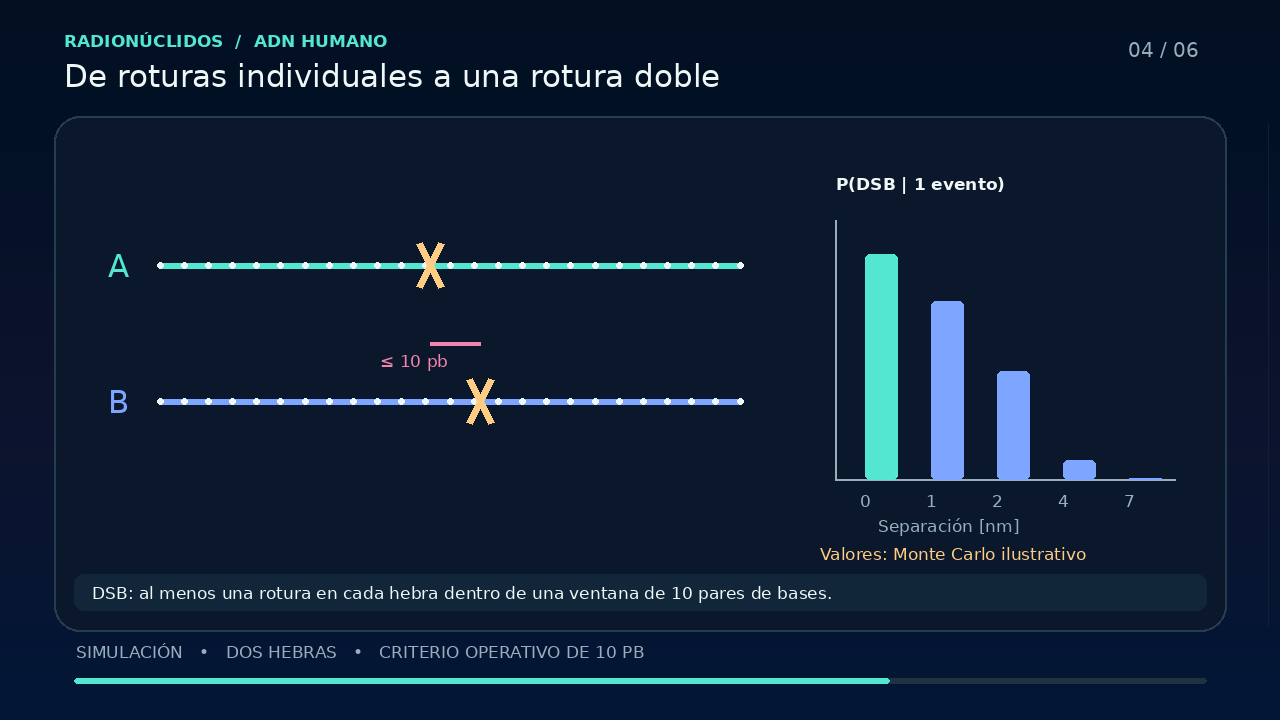
\includegraphics{../media/04_roturas_agrupadas_portada.png}
\caption{La regla sobre dos hebras y un barrido espacial con parámetros del modelo. La gráfica es un resultado simulado; no son datos experimentales.}
\end{figure}

\subsubsection{De energía a dosis: qué representa un gray}\label{de-energuxeda-a-dosis-quuxe9-representa-un-gray}

La energía absorbida \(E_{abs}\) dividida por una masa \(m\) define \(D=E_{abs}/m\) y \(1\,\mathrm{Gy}=1\,\mathrm{J\,kg^{-1}}\). Para un volumen de agua ideal esférico, \(m=\rho(4\pi/3)r^3\). Si \emph{hipotéticamente} se depositara \(1\) keV entero en una esfera de agua de radio \(2\) nm, se obtendría \(E=10^3(1.602176634\times10^{-19})=1.602176634\times10^{-16}\) J, \(m=(10^3\,\mathrm{kg\,m^{-3}})(4\pi/3)(2\times10^{-9}\,\mathrm m)^3=3.3510\times10^{-23}\) kg y \(D\simeq4.78\times10^6\) Gy para \emph{esa masa y ese único evento supuesto}. Ese valor no es una dosis terapéutica, no significa que un electrón real deposite íntegramente 1 keV ahí, y no se compara con una dosis celular promedio sin especificar el volumen y el reparto de energía. Precisamente muestra por qué la escala del volumen debe escribirse cuando se calcula un gray.

\subsection{Después del daño: tres destinos que compiten}\label{despuuxe9s-del-dauxf1o-tres-destinos-que-compiten}

Sea \(L(t)\) la fracción de lesiones aún presentes y \(R(t)\), \(M(t)\), \(C(t)\) las fracciones acumuladas que ya han pasado a reparación, mutación fijada y pérdida celular. El tiempo está en horas y las tasas \emph{hipotéticas} \(k_r=0.20\), \(k_m=0.02\), \(k_c=0.03\) h\(^{-}\)¹. Este \(k_m\) es \emph{otro parámetro} distinto de la pendiente de mutación observada en HPRT. Con \(K=k_r+k_m+k_c=0.25\) h\(^{-}\)¹: \[\frac{dL}{dt}=-KL,\qquad L(0)=1.\]

\[\frac{dR}{dt}=k_rL,\qquad \frac{dM}{dt}=k_mL,\qquad \frac{dC}{dt}=k_cL.\] Integramos: \(L(t)=e^{-Kt}\) y \(R(t)=k_r\int_0^t e^{-Ks}ds=(k_r/K)(1-e^{-Kt})\); sustituyendo \(k_r\) por \(k_m,k_c\) obtenemos \(M(t),C(t)\). Sumando, \[L+R+M+C=e^{-Kt}+\frac{k_r+k_m+k_c}{K}(1-e^{-Kt})=1.\] En el límite \(t\to\infty\) el destino simulado se reparte \(80\%\), \(8\%\), \(12\%\). Son fracciones \emph{asumidas por las tasas}, no prevalencias reales de lesiones ni una calibración humana. ``Mutación fijada'' exige supervivencia y cambios heredables en descendientes celulares: la animación representa la distinción, no reemplaza experimentos de linaje y secuenciación.

\subsection{Del locus HPRT a un conteo interpretable}\label{sec:hprt}

Una rotura observada en ADN no demuestra una mutación heredable; una mutación HPRT se evalúa con una selección y la frecuencia de mutantes entre células clonables. El experimento del artículo registra mutantes en el locus \emph{hprt} y distingue la muerte celular de esta variable {[}1{]}. \textbf{Dos enzimas, dos funciones:} la timidina cinasa (TK) controla la incorporación del análogo IdUrd; la hipoxantina--guanina fosforribosiltransferasa (HPRT) participa en la vía de rescate de purinas y permite seleccionar células resistentes a 6-tioguanina cuando se pierde la función correspondiente. TK6 y SE30 comparan la primera ruta; la medición de mutantes HPRT explora otro locus. No sería correcto afirmar que ``SE30 tiene mutado HPRT'' por ser deficiente en TK. HPRT1 humano se encuentra en el cromosoma X {[}5{]}; O'Neill, Sullivan y Albertini describieron un ensayo de clonación con 6-tioguanina y corrección por capacidad de clonación en células humanas {[}4{]}. Este apoyo metodológico no demuestra que el procedimiento exacto de cultivo de Whaley y Little usara idénticas concentraciones o tiempos.

Si \(n\) células se siembran por pocillo y cada célula tiene probabilidad efectiva \(f\,\varepsilon\) de producir un clon resistente, donde \(f\) es la frecuencia de mutantes y \(\varepsilon\) es su eficiencia de clonación bajo selección, entonces para eventos raros la cantidad de clones resistentes por pocillo se modela como Poisson con media \(nf\varepsilon\). La probabilidad de un pocillo sin clon es \(P_0=e^{-nf\varepsilon}\). Aplicando logaritmo a ambos lados: \(\ln P_0=-nf\varepsilon\), de donde \[\boxed{f=-\frac{\ln P_0}{n\varepsilon}.}\] Esta expresión ilustra por qué contar sólo pocillos positivos no basta: deben conocerse el número sembrado y la eficiencia de clonación, y debe permitirse expresión fenotípica. El programa de esta entrega parte \emph{ya} de un número de células clonables y usa Poisson para ilustrar repeticiones; no reconstruye los datos crudos del artículo.

Para modelar un conteo simplificado con \(n\) células clonables y frecuencia de fondo \(f_0\), usamos \[f_{TK6}(D)=f_0+\alpha D,\qquad \alpha=0.45\times10^{-6}\,\mathrm{cGy}^{-1},\qquad D\ \text{en cGy}.\] La pendiente \(\alpha\) corresponde a ¹³¹IIdUrd en TK6 del artículo; el fondo \(f_0\) no está informado aquí y en la simulación se \emph{elige} \(10\times10^{-6}\). El exceso de frecuencia a \(D=38\) cGy es \[\Delta f=\alpha D=(0.45\times10^{-6}\,\mathrm{cGy}^{-1})(38\,\mathrm{cGy})=17.1\times10^{-6}.\]

Esto equivale a 17,1 mutantes inducidos por millón de células clonables. Además, \(38\,\mathrm{cGy}=0.38\,\mathrm{Gy}\) y \(\alpha=45\times10^{-6}\,\mathrm{Gy}^{-1}\). Se cambió la unidad porque \(1\) Gy \(=100\) cGy; para mantener \(\alpha D\) idéntico, el valor numérico de \(\alpha\) por Gy se multiplica por \(100\). La cifra \(17.1\) es una \textbf{extrapolación de TK6} en un nivel de dosis mencionado para SE30, no una medición directa de TK6 a 38 cGy y tampoco una tasa de mutación del genoma completo. El modelo opcional de réplicas toma \(Y_0\sim\mathrm{Poisson}(nf_0)\) y \(Y_D\sim\mathrm{Poisson}(n(f_0+\alpha D))\); por independencia, \(E[Y_D-Y_0]=n\alpha D\) y \(\mathrm{Var}(Y_D-Y_0)=n(2f_0+\alpha D)\). El número de células \emph{clonables} se presupone, no se infiere de supervivencia.

\subsection{Vínculo preciso con el programa}\label{vuxednculo-preciso-con-el-programa}

Las diapositivas proporcionadas de \emph{Decays and scattering} tratan estados inestables, tasa, semivida, actividad, modos y razón de ramificación: aparecen en las secciones 3--5 {[}10{]}. La presentación \emph{Particle Detection--part 2} introduce pérdida de energía y alcance de partículas en materia: motiva nuestra discusión sobre deposición de energía y límites de un modelo de electrones {[}11{]}. La física de interacciones débiles aparece en la transformación nuclear beta/captura, mientras la relajación electromagnética permite distinguir rayos X, gamma y Auger. No se usan QCD, modelo de capas, Proca o diagramas de Feynman como adornos: no son necesarios para responder esta pregunta. El ensayo HPRT entra como medición biológica posterior y no sustituye una medida de energía de detector.

\subsection{Utilidad, analogías prudentes y limitaciones}\label{utilidad-analoguxedas-prudentes-y-limitaciones}

\textbf{Utilidad científica:} seleccionar blancos subcelulares para estudiar emisores Auger; priorizar medidas de incorporación, distribución y permanencia antes de convertir Bq en efecto; distinguir un biomarcador de daño (roturas) de un desenlace tardío (mutación). \textbf{Símil de actualidad:} una radioterapia con radiofármaco dirigido al núcleo exige saber dónde queda cada fuente; las exposiciones por accidentes nucleares requieren otras vías de entrada, metabolismo y distribución. Los resultados de IdUrd en cultivo no cuantifican las consecuencias sanitarias de Chernóbil, bombas atómicas o radioyodo convencional, ni se extrapolan a personas sin datos de órganos y dosis.

\textbf{Límites del estudio:} (i) las líneas celulares humanas no son una cohorte de pacientes; (ii) la actividad y la dosis al núcleo no identifican por sí solas una secuencia genómica mutada; (iii) la hélice representada contiene 60 pb ideales, no el genoma humano; (iv) el modelo espacial usa un núcleo de probabilidad elegido, independencia de sitios y un criterio operacional DSB; (v) la tasa de residencia, las tasas celulares y el fondo HPRT del código son escenarios; (vi) los vídeos muestran un relato de mecanismos y no mediciones en tiempo real. El experimento de LeMotte y Little encontró aproximadamente una rotura doble por desintegración ¹²⁵I bajo condiciones congeladas {[}3{]}; \emph{esa} medida no valida las probabilidades numéricas de nuestro código para una hélice aislada. La corrección de Schmitz y colaboradores subrayó además que una rotura doble no se convierte automáticamente en aberración cromosómica: sus datos revisados dieron en promedio unas 250 desintegraciones por aberración bajo sus condiciones experimentales {[}9{]}.

\subsection{Síntesis del marco teórico}\label{suxedntesis-del-marco-teuxf3rico}

Las ecuaciones nucleares y la ley de decaimiento describen \emph{cuándo y qué} se emite. La geometría y la permanencia modifican \emph{dónde} se deposita energía. Reparación, supervivencia y selección experimental determinan \emph{qué efecto final se observa}. En cultivos humanos TK6/SE30, Whaley y Little encontraron una diferencia clara entre radionúclidos incorporados y actividad extracelular {[}1{]}. Nuestro modelo muestra una vía consistente para pensar esa diferencia y expone los datos necesarios para verificarla con mayor fidelidad, sin reclamar una predicción clínica o genómica que los datos no sustentan.

\section{Parte II · Desarrollo científico de seis mecanismos}\label{parte-ii-desarrollo-cientuxedfico-de-seis-mecanismos}

\subsection{Capítulo 1. Captura electrónica, transmutación y relajación atómica}\label{capuxedtulo-1.-captura-electruxf3nica-transmutaciuxf3n-y-relajaciuxf3n-atuxf3mica}

El primer nivel de descripción consiste en identificar qué cambia dentro del núcleo. Un isótopo conserva su número de protones \(Z\) y se diferencia por su número de neutrones. El yodo tiene \(Z=53\). En \(^{125}\)I, una transformación por captura electrónica toma un electrón de una capa ligada y convierte un protón nuclear en neutrón. Así, el número de nucleones \(A=125\) permanece constante, mientras el núcleo resultante tiene \(Z=52\) y pertenece al elemento telurio. Escribimos el proceso, omitiendo en esta línea las energías de excitación y retroceso, como

\[\mathrm I(125,53)+e^-_{\mathrm{ligado}}\longrightarrow \mathrm{Te}^{*}(125,52)+\nu_e.\]

La carga inicial total del sistema «núcleo + electrón» es \(+53e-e=+52e\); el núcleo final tiene carga \(+52e\) y el neutrino no lleva carga. El electrón inicial tiene número leptónico electrónico \(+1\) y el neutrino final también. Esta contabilidad evita interpretar la captura como una emisión de electrón beta. La interacción débil gobierna la transformación protón--neutrón. La relajación posterior de la configuración atómica y la conversión interna involucran interacciones electromagnéticas y deben describirse por separado {[}6,10{]}.

Si \(M_a\) indica la masa del átomo neutro en estado fundamental, la energía disponible se define por \(Q_{EC}=[M_a(\mathrm I_{125})-M_a(\mathrm{Te}_{125})]c^2\). Para la captura desde una capa de energía de enlace \(B_i\), y un estado nuclear hijo de excitación \(E_*\), el balance esquemático es

\[Q_{EC}=E_{\nu,i}+E_*+B_i+T_R+\delta_{\mathrm{at}},\]

donde \(T_R\) es el retroceso y \(\delta_{\mathrm{at}}\) representa correcciones atómicas pequeñas según la convención de masas y vacantes usada. Reordenar da \(E_{\nu,i}\simeq Q_{EC}-E_*-B_i-T_R\) cuando se desprecia \(\delta_{\mathrm{at}}\). La igualdad no adjudica a cada electrón Auger una energía igual a \(Q_{EC}\). El neutrino transporta parte de la energía; el núcleo puede desexcitarse por emisión gamma o por conversión interna; la vacante electrónica se rellena mediante radiación característica o transferencia de energía a otro electrón. Cada vacante adicional puede alimentar una nueva transición. La ficha de IAEA para \(^{125}\)I da la semivida y la línea gamma de aproximadamente 35,49 keV con intensidad minoritaria {[}6{]}. Una línea gamma nuclear no es la energía común de los electrones Auger.

La posición inicial del núcleo hijo coincide con la posición del padre en el instante de la transformación dentro de la precisión de escala molecular pertinente. Esto permite afirmar que las emisiones y la relajación comienzan localmente si el padre estaba en ADN. No permite afirmar que Te permanezca químicamente enlazado después de la ionización múltiple, ni que los electrones sigan trayectorias radiales rectas. En Whaley y Little, el contraste central no es la persistencia del enlace del hijo, sino la diferencia de efecto entre desintegraciones de un análogo incorporado y actividad extracelular {[}1{]}.

\begin{figure}[htbp]
\centering
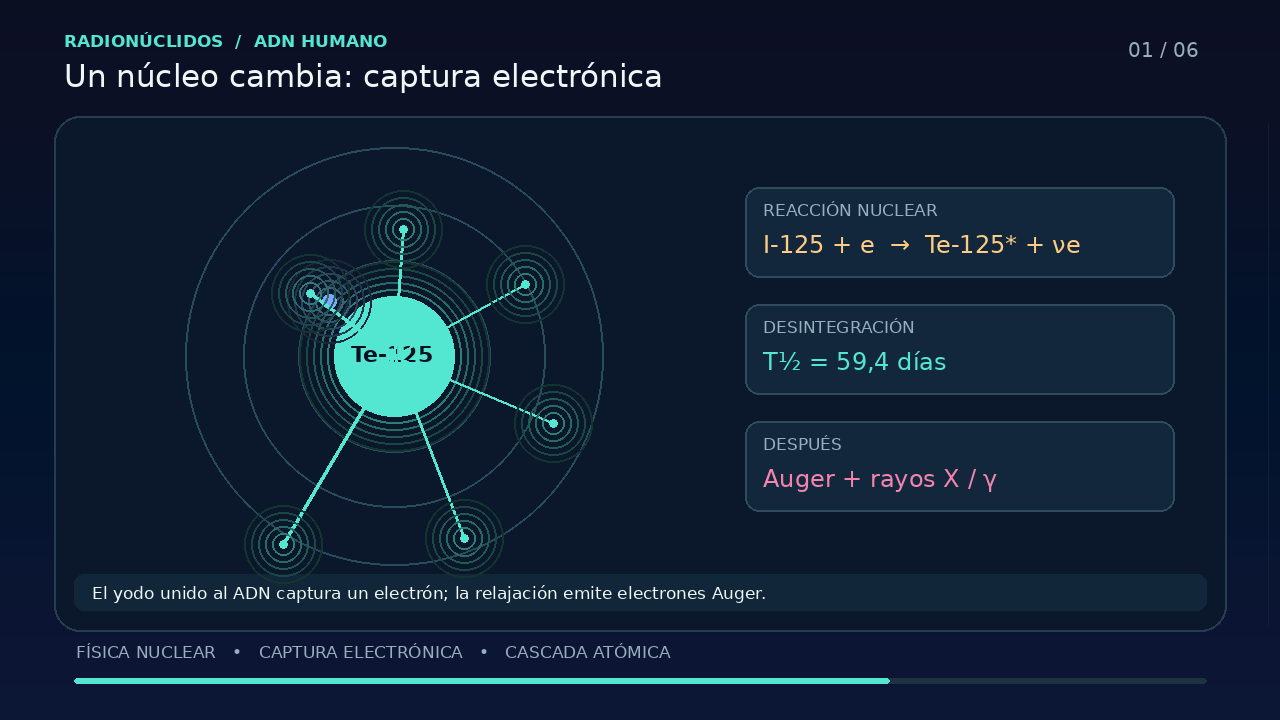
\includegraphics{../media/01_captura_y_Auger_portada.png}
\caption{Esquema narrativo original de captura y cascada; no representa un espectro medido}
\end{figure}

\subsection{Capítulo 2. Dos escalas temporales: desintegración y permanencia}\label{capuxedtulo-2.-dos-escalas-temporales-desintegraciuxf3n-y-permanencia}

Para derivar la ley nuclear no se presupone que todos los átomos decaigan en un momento único. Se supone una probabilidad condicional \(\lambda\,dt+o(dt)\) de que un átomo todavía no desintegrado decaiga entre \(t\) y \(t+dt\), con \(\lambda\) constante. En un conjunto de \(N(t)\) núcleos, el número medio de pérdidas en ese intervalo es \(\lambda N(t)dt\). Se obtiene sucesivamente

\[N(t+dt)-N(t)=-\lambda N(t)dt+o(dt),\]

\[\frac{dN}{dt}=-\lambda N,\qquad \frac{dN}{N}=-\lambda dt,\]

\[\ln N(t)-\ln N_0=-\lambda t,\qquad N(t)=N_0e^{-\lambda t}.\]

La semivida se define por \(N(T_{1/2})/N_0=1/2\). Por tanto \(\exp(-\lambda T_{1/2})=1/2\), de donde \(-\lambda T_{1/2}=-\ln2\) y finalmente \(\lambda=\ln2/T_{1/2}\). La vida media temporal \(\tau_n=1/\lambda\) no coincide con la semivida: \(\tau_n=T_{1/2}/\ln2\). La actividad \(A=-dN/dt=\lambda N\) es positiva. Cuando \(\lambda\) se ha obtenido en días\(^{-1}\), la actividad en Bq requiere dividir la tasa por 86 400 segundos/día. Las semividas físicas tabuladas de 59,40 y 8,021 días para \(^{125}\)I y \(^{131}\)I, respectivamente, proceden de ICRP {[}7{]}.

Ahora se introduce un segundo mecanismo: un átomo incorporado puede abandonar el compartimento que llamamos «ADN» antes de decaer. Si la salida es exponencial con riesgo constante \(k\) por día e independiente del mecanismo nuclear, la fracción que todavía está incorporada y sin decaer al tiempo \(t\) cumple \(dn/dt=-(\lambda+k)n\). La solución \(n(t)=n_0e^{-(\lambda+k)t}\) describe la población que conserva ambas condiciones. El número medio de decaimientos locales que ocurre en un intervalo \(dt\) es \(\lambda n(t)dt\). Al integrar desde 0 hasta \(t\) y dividir por \(n_0\),

\[P_{\mathrm{local}}(t)=\frac{1}{n_0}\int_0^t\lambda n_0e^{-(\lambda+k)s}ds
=\frac{\lambda}{\lambda+k}\left(1-e^{-(\lambda+k)t}\right).\]

El límite de tiempo largo es \(P_{\mathrm{local}}(\infty)=\lambda/(\lambda+k)\). Si se habla de \textbf{residencia media} \(\tau_b\), la tasa correspondiente es \(k=1/\tau_b\); sólo si se hablara de una \emph{semivida biológica} sería \(k=\ln2/T_{b,1/2}\). Confundir esos dos tiempos introduciría un factor \(\ln2\) erróneo. Para \(\tau_b=2\) días elegidos hipotéticamente, \(k=0.5\) d\(^{-1}\) y resultan \(P_{125}=0.022806\) y \(P_{131}=0.147364\). El segundo átomo tiene, en ese esquema de salida, mayor posibilidad de desintegrarse antes de abandonar el ADN por su semivida nuclear más corta; la intensidad del daño \textbf{por decaimiento local} sigue siendo otra pregunta. Este modelo no ajusta una cinética biológica de las líneas TK6 o SE30.

\begin{figure}[htbp]
\centering
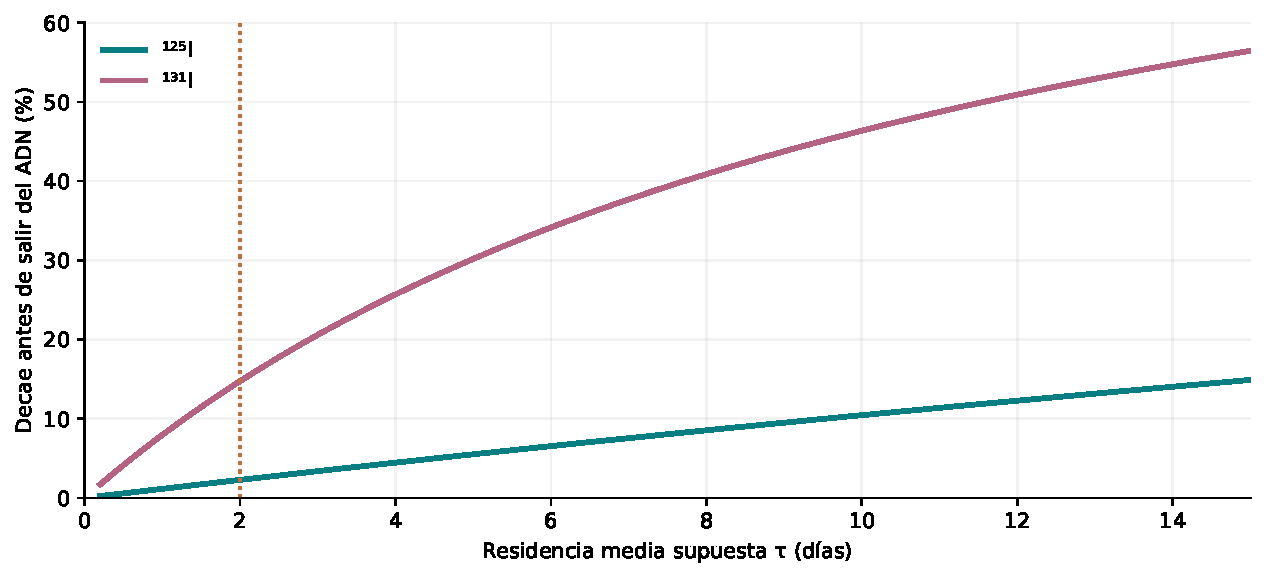
\includegraphics{figuras_monografia/03_retencion_hipotetica.pdf}
\caption{Predicción de los dos riesgos en función de una residencia media supuesta}
\end{figure}

\subsection{Capítulo 3. Geometría del ADN y ley fenomenológica de lesión}\label{capuxedtulo-3.-geometruxeda-del-adn-y-ley-fenomenoluxf3gica-de-lesiuxf3n}

La proximidad requiere una definición geométrica y una unidad. «Diez pares de bases» cuenta posiciones sucesivas en la secuencia; «diez nanómetros» expresa una longitud. En la representación ideal escogida, el avance axial es \(h=0.34\) nm por par, de modo que una separación de diez índices corresponde a 3,4 nm \textbf{axiales}. Las hebras se sitúan también a distintas coordenadas transversales. Se modelan 60 posiciones por hebra y una vuelta cada diez pares de bases. Para \(j\in\{0,\ldots,59\}\) se fija

\[\theta_j=\frac{2\pi(j-30)}{10},\qquad z_j=0.34(j-30)\,\mathrm{nm}.\]

Con un radio \(R=1\) nm, las coordenadas de las dos columnas ideales son \(\mathbf x_{A,j}=(R\cos\theta_j,R\sin\theta_j,z_j)\) y \(\mathbf x_{B,j}=(-R\cos\theta_j,-R\sin\theta_j,z_j)\). El código ubica la fuente en \(\mathbf s=(R+d,0,0)\), con \(d\geq0\) en nm. Para cada sitio, \(r_{X,j}=\|\mathbf x_{X,j}-\mathbf s\|\) se calcula mediante la raíz de la suma de cuadrados de las tres diferencias de coordenadas. Si \(d=0\), \(\mathbf x_{A,30}=\mathbf s\) y \(r_{A,30}=0\), mientras \(r_{B,30}=2R=2\) nm. Es una comprobación de geometría del código, no la distancia de un átomo real a una estructura atómica resuelta.

Se necesita convertir las distancias en probabilidades para simular lesiones. El proyecto elige un peso \(q(r)=\exp(-r/\ell)\), donde \(\ell>0\) controla qué tan rápido decrece el peso. La función no es un espectro de electrones ni la ley de atenuación de un material macroscópico. Postulamos que en un sitio existen oportunidades de rotura con conteo Poisson de media \(\mu q(r)\), con \(\mu\geq0\) adimensional. En una Poisson de media \(a\), \(P(K=0)=e^{-a}\). Por complemento,

\[P(K\geq1)=1-P(K=0)=1-e^{-a}
=1-\exp\left[-\mu\exp(-r/\ell)\right].\]

Esta última expresión define \(p_{X,j}\) para cada hebra y cada índice. En \(r=0\) vale \(1-e^{-\mu}\) y cuando \(r\to\infty\) tiende a cero. Para valores pequeños de \(\mu q\), la expansión \(e^{-x}=1-x+O(x^2)\) da \(p\simeq\mu e^{-r/\ell}\); cuando \(\mu\) crece mucho, \(p\) se satura hacia uno y deja de aumentar linealmente. Martin y Haseltine {[}2{]} observaron la mayor parte del daño a 15--20 Å y roturas detectables hasta 70 Å en otro sistema experimental. Esa observación motiva una pregunta espacial, pero no determina \(\ell=1.5\) nm ni \(\mu=0.48\) utilizados en la figura. No se ha ajustado ninguno de ellos a datos del artículo guía.

\begin{figure}[htbp]
\centering
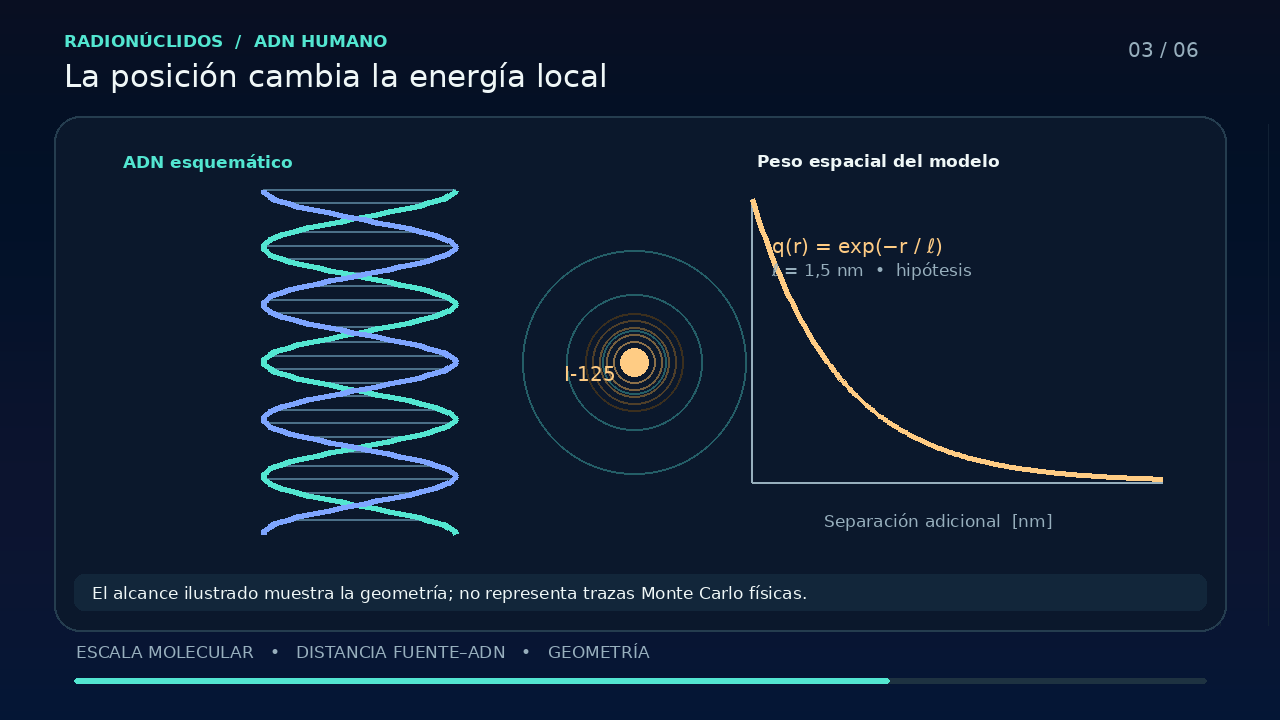
\includegraphics{../media/03_distancia_fuente_ADN_portada.png}
\caption{Esquema de hélice ideal y distancia de la fuente}
\end{figure}

\subsection{Capítulo 4. De roturas simples a una rotura doble operacional}\label{capuxedtulo-4.-de-roturas-simples-a-una-rotura-doble-operacional}

Una variable de Bernoulli toma los valores 0 o 1. Para cada sitio simulado, el programa obtiene un uniforme \(U_{X,j}\) entre cero y uno y define \(B_{X,j}=1\) si \(U_{X,j}<p_{X,j}\), o \(B_{X,j}=0\) en otro caso. Condicionadas a los parámetros fijos, estas variables se sortean independientemente. Una rotura simple queda representada por un 1 en una hebra. La simplificación separa los sitios matemáticamente, aunque una cascada real puede producir daños correlacionados por electrones, radicales y estructura de cromatina.

La DSB de este trabajo es una variable indicadora de evento. Vale 1 exactamente si \textbf{existe} al menos una pareja de posiciones \((i,j)\) tales que \(B_{A,i}=B_{B,j}=1\) y \(|i-j|\leq10\). Vale cero si no existe tal pareja. Una rotura en A20 y otra en B30 da distancia de índices 10 y cumple la regla; B31 produciría 11 y no la cumple. Dos roturas en la misma hebra no la cumplen. La expresión «existe» importa porque un evento puede contener numerosas parejas: el programa cuenta una sola vez que \textbf{hubo} DSB y no confunde el número de parejas con la probabilidad del evento.

Para \(n\) repeticiones del mismo escenario se define \(I_k\in\{0,1\}\) como resultado del evento \(k\). El estimador es \(\widehat p=n^{-1}\sum_{k=1}^{n}I_k\). Bajo independencia entre repeticiones, \(E(\widehat p)=p\) y \(\mathrm{Var}(\widehat p)=p(1-p)/n\). Se reemplaza \(p\) por \(\widehat p\) para informar \(SEM=\sqrt{\widehat p(1-\widehat p)/n}\). El «intervalo» \(\widehat p\pm1.96SEM\) es una aproximación normal de incertidumbre \textbf{de muestreo}; si \(p\) está muy cerca de cero o uno, conviene un intervalo de Wilson o exacto. No cubre el error de un modelo físico inadecuado.

Hay un control independiente para «alguna rotura». Dado que cada sitio se sortea de manera independiente, la probabilidad de no romper ninguno es \(\prod_{X,j}(1-p_{X,j})\); por complemento \(P(\text{alguna rotura})=1-\prod_{X,j}(1-p_{X,j})\). Para DSB no basta multiplicar probabilidades de parejas y sumar: dos o más parejas pueden coexistir. El algoritmo busca si aparece al menos una pareja y repite miles de veces. Con 15 000 eventos por distancia y semilla 2026, el escenario base da \(\widehat p_{DSB}(0)=0.8700\) y \(\widehat p_{DSB}(4)=0.0718\). Como cambiar \(\mu\) y \(\ell\) modifica mucho esos valores, no se interpretan como rendimientos biológicos universales.

\begin{figure}[htbp]
\centering
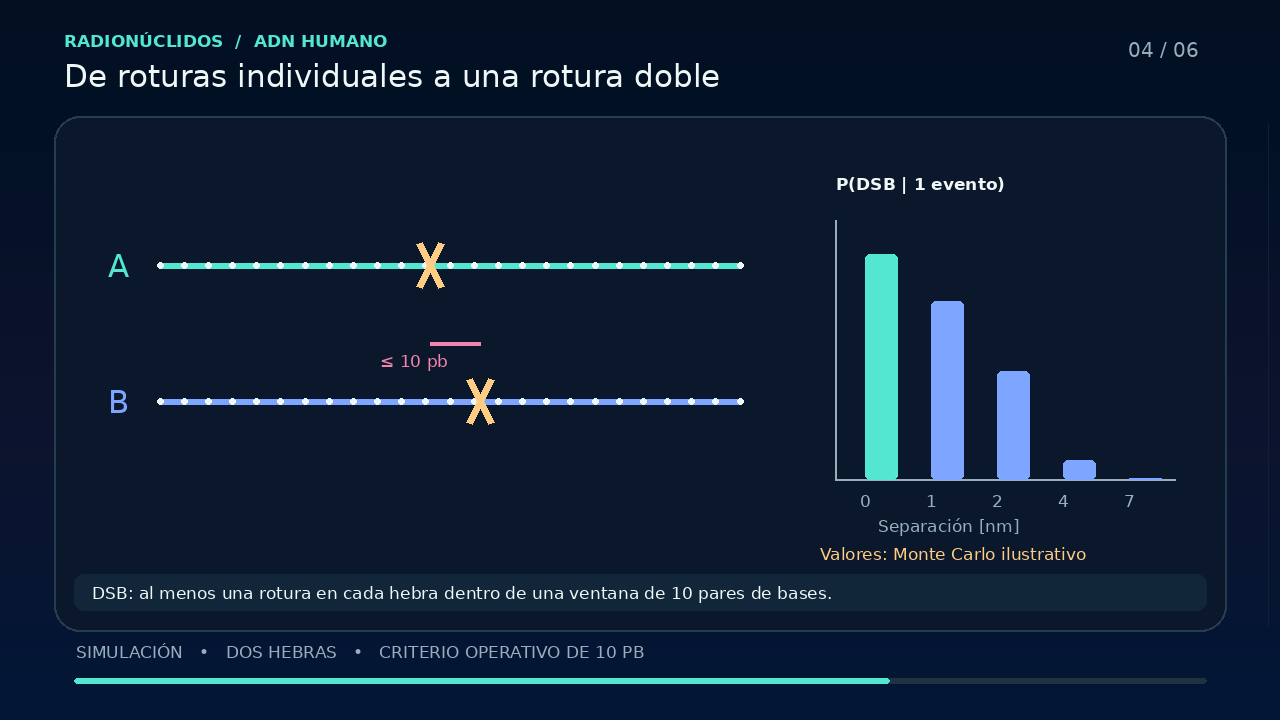
\includegraphics{../media/04_roturas_agrupadas_portada.png}
\caption{Definición operacional de pareja en dos hebras}
\end{figure}

\begin{figure}[htbp]
\centering
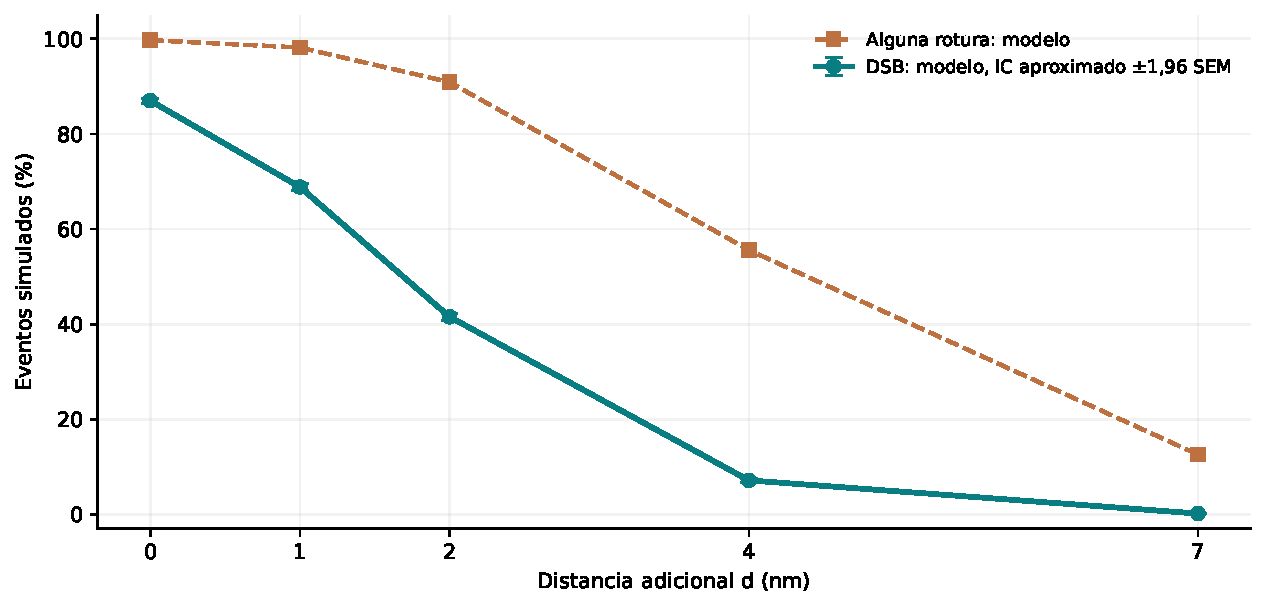
\includegraphics{figuras_monografia/01_distancia_y_roturas.pdf}
\caption{Estimaciones del Monte Carlo según distancia, con error de muestreo}
\end{figure}

\subsection{Capítulo 5. Cinética de lesión, reparación y destinos competidores}\label{capuxedtulo-5.-cinuxe9tica-de-lesiuxf3n-reparaciuxf3n-y-destinos-competidores}

La ocurrencia de un daño no equivale a una mutación detectada. Una célula puede reparar la lesión, fijar un cambio heredable en una descendencia clonable o perderse del conjunto que se puede evaluar. La simulación representa estas alternativas con un estado inicial \(L(0)=1\) y tres salidas acumuladas \(R(0)=M(0)=C(0)=0\). Se postulan riesgos constantes no negativos \(k_r\), \(k_m\) y \(k_c\) por hora y se define \(K=k_r+k_m+k_c\). En un intervalo \(dt\), la lesión no resuelta pierde una fracción \(KLdt\). Por ello

\[\frac{dL}{dt}=-KL,\qquad L(t)=e^{-Kt}.\]

La probabilidad acumulada de reparación cambia a razón \(dR/dt=k_rL(t)\). Integrando desde cero,

\[R(t)=\int_0^tk_re^{-Ks}ds
=\frac{k_r}{K}\left(1-e^{-Kt}\right).\]

Con idéntico procedimiento se obtienen \(M(t)=k_m(1-e^{-Kt})/K\) y \(C(t)=k_c(1-e^{-Kt})/K\). La conservación se demuestra sin datos empíricos: \(L+R+M+C=e^{-Kt}+(k_r+k_m+k_c)(1-e^{-Kt})/K=1\). El tiempo característico de resolución del estado inicial es \(1/K\). Para \(k_r=0.20\), \(k_m=0.02\) y \(k_c=0.03\) h\(^{-1}\) elegidos, \(K=0.25\) h\(^{-1}\) y \(1/K=4\) h. Al tomar \(t\to\infty\), las fracciones resultan 0,80, 0,08 y 0,12. Éstas se fijaron indirectamente al elegir las tasas; no son frecuencias medidas de los cultivos del artículo {[}1{]}.

La variable \(M\) debe leerse como estado de «fijación» dentro de un esquema matemático. Para demostrar una mutación experimental hay que dejar transcurrir expresión fenotípica, corregir supervivencia y selección, y analizar clones. Una DSB puede repararse fielmente, repararse con cambio, participar en un reordenamiento o impedir la clonación. Por eso no se multiplica la probabilidad DSB simulada por \(0.08\) y se afirma haber predicho la frecuencia de HPRT. Las dos cantidades provienen de módulos con supuestos diferentes y sin calibración conjunta.

\begin{figure}[htbp]
\centering
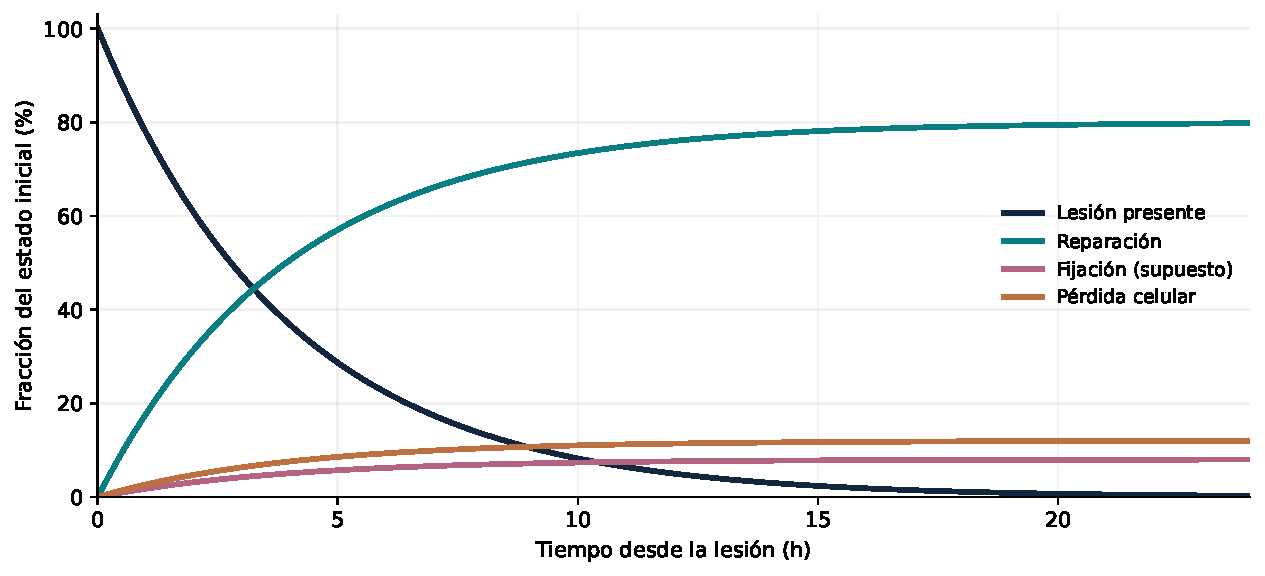
\includegraphics{figuras_monografia/02_destinos_celulares.pdf}
\caption{Estados celulares acumulados bajo tasas ilustrativas}
\end{figure}

\subsection{Capítulo 6. Ensayo HPRT: diseño celular, dosis y estadística del recuento}\label{capuxedtulo-6.-ensayo-hprt-diseuxf1o-celular-dosis-y-estaduxedstica-del-recuento}

La pregunta experimental exige separar la vía de incorporación de la variable de salida. La timidina cinasa (TK) permite incorporar el análogo nucleosídico mediante la ruta de salvamento de timidina. TK6 es competente y SE30 es deficiente para esa capacidad en el diseño descrito por Whaley y Little {[}1{]}. Esta comparación cambia la probabilidad de situar la fuente en el ADN. En cambio, \emph{hprt} designa un locus distinto: HPRT participa en el rescate de purinas y puede utilizarse en la selección de clones resistentes a 6-tioguanina cuando se pierde función. HPRT1 humano está en el cromosoma X {[}4,5{]}. La deficiencia de TK en SE30 no significa que HPRT sea la misma enzima o que todos sus clones ya sean HPRT mutantes.

En un ensayo de clonación idealizado, si se siembran \(n\) células por pocillo, cada una tiene frecuencia \(f\) de fenotipo resistente y probabilidad \(\varepsilon\) de generar una colonia bajo selección. Para eventos raros e independientes se aproxima el número de clones resistentes por Poisson de media \(nf\varepsilon\). La probabilidad de no observar colonia es \(P_0=e^{-nf\varepsilon}\). Al tomar logaritmo y despejar,

\[\ln P_0=-nf\varepsilon,\qquad f=-\frac{\ln P_0}{n\varepsilon}.\]

Así se hace visible por qué el número de células sembradas y la eficiencia de clonación importan. La ecuación describe un mecanismo de lectura posible, no reconstruye los pocillos específicos del artículo de Whaley y Little. La frecuencia mutante se estima entre células capaces de crecer bajo condiciones apropiadas; la muerte celular es otro resultado experimental {[}1,4{]}.

El resumen público de Whaley y Little informa una pendiente inducida de \(\alpha=0.45\times10^{-6}\) mutantes HPRT por cGy de dosis nuclear para \(^{131}\)I--IdUrd en células TK competentes {[}1{]}. El mismo resumen señala pocas mutaciones en células TK deficientes hasta 38 cGy cuando las desintegraciones de \(^{131}\)I ocurren en el medio. Para explorar unidades se define \(f(D)=f_0+\alpha D\). El fondo \(f_0=10\times10^{-6}\) usado en el código es una hipótesis didáctica. En \(D=38\) cGy, el exceso \textbf{calculado} sería \(\alpha D=17.1\times10^{-6}\), equivalente a 17,1 por millón de células clonables; no se presenta como dato TK6 medido exactamente a 38 cGy. La dosis es una energía absorbida por masa: \(1\) Gy = \(1\) J/kg y \(1\) Gy = 100 cGy. La pendiente numérica por Gy correspondiente es \(45\times10^{-6}\), porque \(\alpha_{Gy}(0.38\,Gy)=\alpha_{cGy}(38\,cGy)\).

El recuento ilustrativo usa \(Y_0\sim\mathrm{Poisson}(nf_0)\) y \(Y_D\sim\mathrm{Poisson}(n[f_0+\alpha D])\). Si ambos son independientes, \(E(Y_D-Y_0)=n\alpha D\) y \(\mathrm{Var}(Y_D-Y_0)=n(2f_0+\alpha D)\). Con \(n=10^6\) y el fondo supuesto, las medias son 10 y 27,1, pero un par de recuentos generados puede diferir de esas medias. El proyecto no reestima \(\alpha\) ni su incertidumbre a partir de datos crudos. Una extrapolación lineal tampoco permite convertir mutantes HPRT en riesgo de cáncer, secuencia de todo el genoma o frecuencia de mutación humana individual.

\begin{figure}[htbp]
\centering
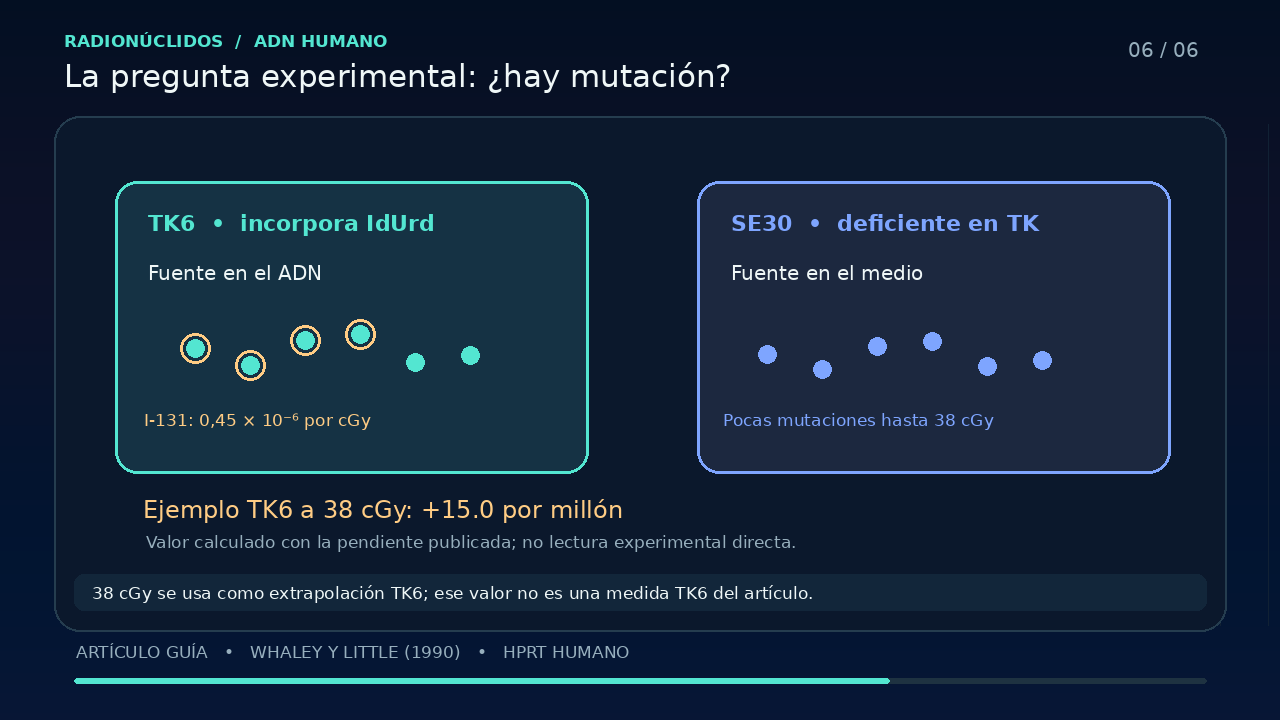
\includegraphics{../media/06_experimento_HPRT_portada.png}
\caption{Comparación conceptual de las dos líneas celulares y la selección HPRT}
\end{figure}

\begin{figure}[htbp]
\centering
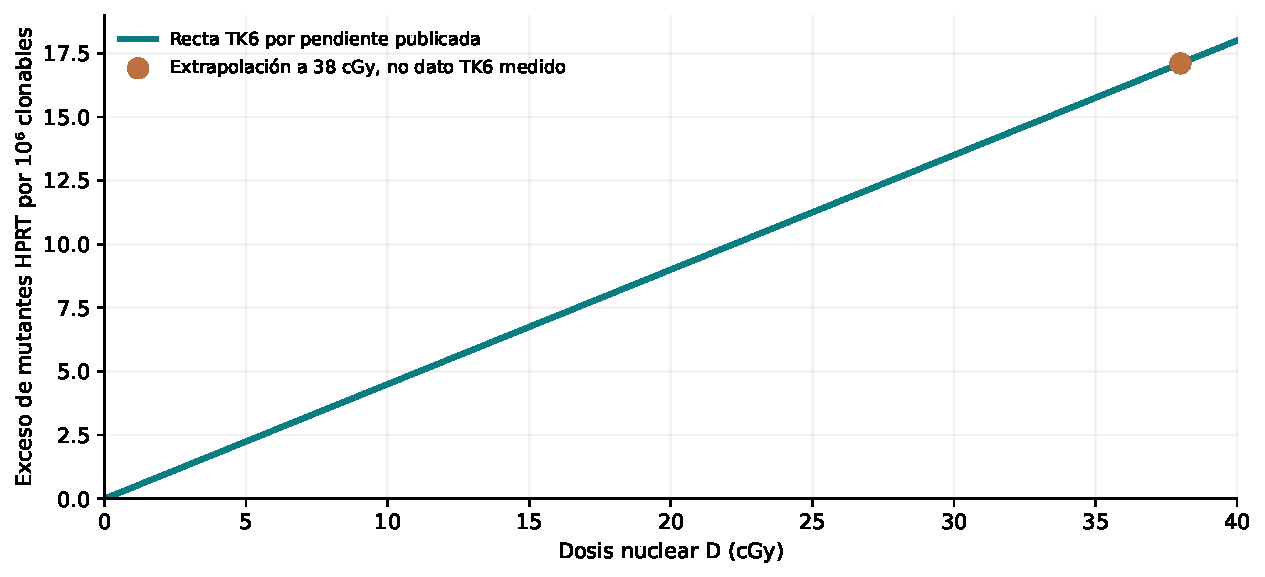
\includegraphics{figuras_monografia/04_hprt_extrapolacion.pdf}
\caption{Pendiente experimental informada y punto extrapolado a 38 cGy}
\end{figure}

\section{Parte III · Resultados, implementación y crítica}\label{parte-iii-resultados-implementaciuxf3n-y-cruxedtica}

\subsection{Arquitectura de cálculo y correspondencia entre los dos programas}\label{arquitectura-de-cuxe1lculo-y-correspondencia-entre-los-dos-programas}

\path{python/modelo.py} define constantes, funciones puras, geometría y muestreo; \path{python/verificar.py} controla casos límite, unidades y reproducibilidad. \texttt{science.js} reproduce las ecuaciones para navegador con otro generador pseudoaleatorio; \texttt{lab.js} conecta los deslizadores y dibuja el Canvas. \texttt{python/animar.py} crea seis vídeos pregrabados y portadas a partir de gráficos narrativos; \textbf{un MP4 no cambia cuando se mueven los controles}, mientras el Canvas sí. La visualización web ejecuta normalmente 3500 eventos por configuración; la tabla de referencia guardada por Python ejecutó 15 000 por distancia. Los porcentajes no tienen por qué coincidir al último decimal. Ambos programas usan la misma definición de lesión, pero NumPy y JavaScript no comparten secuencia de números aleatorios.

\textbf{Pseudocódigo exacto del núcleo Monte Carlo:}

\begin{verbatim}
Entrada: d, μ, ell, n, semilla.
Calcular 60 coordenadas para cada una de las dos hebras.
Para cada hebra y sitio: r = distancia 3D a la fuente; p = 1 − exp(−μ exp(−r/ell)).
Crear n pares de vectores de 60 uniformes independientes con la semilla.
Para cada evento k: rotura_A[j] = (U_A[k,j] < p_A[j]); análogo en B.
Registrar una rotura cualquiera si existe al menos un sitio marcado.
Registrar DSB si existen i,j marcados en hebras opuestas con |i−j| \(\leq\) 10.
Retornar proporciones por n y SEM = sqrt(p̂(1−p̂)/n).
\end{verbatim}

Python genera una matriz común de uniformes para comparar distancias en una misma corrida. Esa correlación reduce el ruido de \emph{diferencias entre escenarios}; el SEM mostrado para una proporción individual sigue siendo binomial. Para una comprobación analítica independiente, la independencia de Bernoulli por sitio implica \(P(\text{alguna})=1-\prod_j(1-p_{A,j})\prod_j(1-p_{B,j})\). No hay una fórmula simple usada por el programa para el criterio de pareja DSB; se estima por muestreo.

\subsection{Tabla reproducible del escenario principal}\label{tabla-reproducible-del-escenario-principal}

Parámetros fijos: 60 pb, \(R=1\) nm, 10 pb/vuelta, \(\mu=0.48\), \(\ell=1.5\) nm, criterio de separación \(\leq10\) pb, semilla NumPy 2026 y \(n=15,000\) eventos por distancia. Resultados extraídos del JSON del repositorio:

\begin{longtable}[]{@{}rrrrr@{}}
\toprule\noalign{}
d (nm) & P(al menos una rotura) & P(DSB) & SEM de P(DSB) & Eventos \\
\midrule\noalign{}
\endhead
\bottomrule\noalign{}
\endlastfoot
0 & 0,99713 & 0,87000 & 0,00275 & 15 000 \\
1 & 0,98167 & 0,68847 & 0,00378 & 15 000 \\
2 & 0,90880 & 0,41560 & 0,00402 & 15 000 \\
4 & 0,55587 & 0,07180 & 0,00211 & 15 000 \\
7 & 0,12580 & 0,00200 & 0,00036 & 15 000 \\
\end{longtable}

\textbf{Lectura:} el intervalo normal aproximado al 95 \% sería \(\widehat p\pm1.96\,SEM\) cuando funciona la aproximación; cerca de cero conviene Wilson o binomial exacto. El error de Monte Carlo no incluye la incertidumbre de \(\mu\), \(\ell\), la independencia por sitio ni la validez de la geometría.

\subsection{Sensibilidad: los parámetros importan más que el ruido numérico}\label{sensibilidad-los-paruxe1metros-importan-muxe1s-que-el-ruido-numuxe9rico}

Cada fila siguiente usa 6000 eventos en Python, semilla 2026. Al variar una hipótesis, se mantienen las otras en su valor base.

\begin{longtable}[]{@{}lrr@{}}
\toprule\noalign{}
Variación del modelo & P(DSB), d=0 nm & P(DSB), d=4 nm \\
\midrule\noalign{}
\endhead
\bottomrule\noalign{}
\endlastfoot
\(\mu=0.24\), \(\ell=1.5\) nm & 0,53083 & 0,02167 \\
\(\mu=0.96\), \(\ell=1.5\) nm & 0,99333 & 0,21467 \\
\(\mu=0.48\), \(\ell=1.0\) nm & 0,59250 & 0,00317 \\
\(\mu=0.48\), \(\ell=2.0\) nm & 0,96250 & 0,30033 \\
\end{longtable}

La distancia tiene un efecto cualitativo robusto dentro de estas elecciones, pero las magnitudes cambian fuertemente. No se ajustó ningún parámetro a un número experimental de DSB. Una predicción cuantitativa requeriría espectros de emisión, transporte a nanoescala, entorno químico, localización real y validación con datos.

\subsection{Verificaciones funcionales y límites de lo probado}\label{verificaciones-funcionales-y-luxedmites-de-lo-probado}

Se ejecutaron con éxito los cinco controles de \path{python/verificar.py}, ocho pruebas de \path{tests/science.test.mjs} y la comprobación de 153 enlaces o recursos locales en siete HTML. Esas pruebas verifican, entre otros aspectos: \(N(T_{1/2})=N_0/2\); signo de actividad; competencia temporal y límites; radio y avance de hélice; umbral de 10 frente a 11 pb; semilla reproducible; comparación analítica de alguna rotura; conservación de cuatro destinos; conversión cGy/Gy y el cálculo 17,1. El sitio utiliza HTML/CSS/JavaScript estáticos con Canvas 2D, sin servidor de cálculo ni base de datos. El visor ofrece texto alternativo y controles etiquetados; los vídeos MP4 pueden pausarse. Una prueba automatizada no sustituye leer y evaluar el artículo completo ni valida el modelo contra nuevos experimentos.

\textbf{Comandos, desde la raíz del repositorio:}

\begin{verbatim}
python -m pip install -r python/requirements.txt
python python/verificar.py
node --test tests/science.test.mjs
python tests/check_links.py
python python/modelo.py
python -m http.server 8000
\end{verbatim}

El último comando permite abrir \texttt{http://localhost:8000/}; el sitio publicado está en \href{https://morganestampadoscol.github.io/radiogenoma-subatomica/}{GitHub Pages}. \path{python/modelo.py} crea \path{resultados/resumen_modelo.json}; el JSON de referencia ya generado reside en \texttt{documentacion/resumen\_modelo.json}. Las seis portadas y los MP4 se entregan en \texttt{media/} y se regeneran con \texttt{python\ python/animar.py} si están instalados sus requisitos y FFmpeg.

\subsection{Alcance del resultado y conclusión}\label{alcance-del-resultado-y-conclusiuxf3n}

\textbf{{[}DATO{]}} TK6 y SE30 permiten estudiar el efecto de incorporar IdUrd radiactiva en ADN sobre muerte celular y HPRT bajo condiciones de cultivo {[}1{]}. \textbf{{[}MODELO{]}} La dependencia de distancia, la regla DSB, los destinos y la residencia son hipótesis explícitas que ayudan a pensar la causalidad. \textbf{{[}EXTRAPOLACIÓN{]}} La pendiente TK6 multiplicada por 38 cGy produce 17,1 por millón, pero ese punto no fue informado como medición TK6 en el resumen {[}1{]}. Ni la simulación ni el artículo permiten calcular mutación de todo el genoma, pronóstico clínico, riesgo de una persona expuesta o efecto de un accidente nuclear. El aporte académico está en construir una cadena explicativa verificable y reconocer dónde termina cada evidencia.

\subsection{Glosario y comprobación de unidades}\label{glosario-y-comprobaciuxf3n-de-unidades}

\begin{longtable}[]{@{}
  >{\raggedright\arraybackslash}p{(\columnwidth - 2\tabcolsep) * \real{0.5000}}
  >{\raggedright\arraybackslash}p{(\columnwidth - 2\tabcolsep) * \real{0.5000}}@{}}
\toprule\noalign{}
\begin{minipage}[b]{\linewidth}\raggedright
Término
\end{minipage} & \begin{minipage}[b]{\linewidth}\raggedright
Significado en este trabajo
\end{minipage} \\
\midrule\noalign{}
\endhead
\bottomrule\noalign{}
\endlastfoot
Bq & Una desintegración por segundo; actividad, no dosis. \\
Gy y cGy & Energía absorbida por masa, 1 Gy = 1 J/kg = 100 cGy. \\
SSB / DSB & Rotura simple / criterio operativo de roturas en hebras opuestas. \\
pb & Par de bases; 10 pb equivalen aproximadamente a 3,4 nm longitudinales en la hélice ideal. \\
TK / HPRT & Timidina cinasa para incorporación del análogo / enzima distinta cuyo locus se evalúa con mutantes resistentes. \\
SEM & Error estándar de la proporción Monte Carlo, no incertidumbre total del modelo. \\
\(\mu\), \(\ell\) & Oportunidades de daño (adimensional) y longitud de perfil (nm), elegidas. \\
\(\lambda\), \(k\) & Tasas de decaimiento y de salida, ambas en d\(^{-}\)¹ en la escena 02. \\
\(k_r,k_m,k_p\) & Tasas ilustrativas de destinos, en h\(^{-}\)¹ en la escena 05. \\
\end{longtable}

\clearpage
\section{Parte IV · Desarrollo físico, evidencia humana y cálculos ampliados}
\label{parte-ampliada}

Los capítulos anteriores describen exactamente lo que ejecuta el atlas interactivo.
Esta parte amplía el contexto científico de la monografía de referencia aportada por
los autores. Sus cálculos adicionales se identifican como \emph{análisis en papel}:
el navegador no evalúa un espectro beta, no transporta electrones y no estima una
dosis individual. Esta distinción permite estudiar con profundidad la física de
$^{125}$I y $^{131}$I sin atribuir a la aplicación capacidades que no tiene.

\subsection{Capítulo 7. El sistema biológico y el control experimental}
\label{ampliacion-sistema}

\subsubsection{Incorporación de un análogo de timidina}
El yodo de la iododesoxiuridina, llamada IUdR o IdUrd según la nomenclatura de
cada artículo, forma parte de una molécula análoga a un nucleósido. Durante la
síntesis de ADN, una célula que capta y fosforila el análogo puede incorporarlo
a la cadena naciente. Por tanto, \emph{exposición a actividad en un tubo de cultivo}
y \emph{decaimiento desde la molécula de ADN} no son la misma condición física.
La primera depende de la cantidad en el medio; la segunda exige captación,
metabolismo e incorporación. Tampoco toda célula de una población está en la
misma fase del ciclo ni contiene el mismo número de moléculas marcadas. El
promedio de actividad de la placa puede esconder una distribución desigual entre
células y entre compartimentos de una misma célula.

Whaley y Little emplearon dos líneas linfoblastoides humanas. TK6 era competente
para incorporar el análogo por la vía dependiente de timidina cinasa; SE30 era
deficiente en esa capacidad [1]. Esta diferencia opera como control de
localización, aunque no autoriza a asumir que las líneas son idénticas en todos
los aspectos. Los autores consideraron explicaciones alternativas, como
sensibilidades radiológicas o sensibilización por el análogo, y concluyeron que
no explicaban la diferencia observada [1]. En particular, el $^{125}$I--IdUrd
incorporado fue muy tóxico y mutagénico en TK6, mientras una actividad semejante
en el medio externo casi no produjo efecto en las células deficientes. Para
$^{131}$I--IdUrd se comunicó en TK6 una pendiente de mutantes inducidos en
\emph{hprt} de $0,45\times10^{-6}$ por cGy de dosis nuclear; se encontraron
pocas mutaciones en SE30 hasta 38 cGy provenientes de decaimientos del medio
[1]. No se publicó allí una tasa universal de mutación de todo el genoma.

El resultado permite una inferencia física importante. Si dos preparaciones
tienen actividad macroscópica comparable, pero una inicia emisiones directamente
en el ADN, la topología microscópica de la fuente modifica la probabilidad de
que una traza intercepte moléculas relevantes. No se deduce que cada desintegración
cause una lesión, que cada lesión se convierta en mutación ni que los valores
obtenidos en cultivo puedan aplicarse sin más a pacientes.

\subsubsection{Qué mide HPRT y qué significa un clon resistente}
La hipoxantina--guanina fosforribosiltransferasa participa en la vía de rescate de
purinas. La selección con 6-tioguanina puede enriquecer células que perdieron
función HPRT y sobreviven bajo las condiciones del ensayo. La timidina cinasa
interviene en la incorporación del análogo: no debe confundirse con HPRT,
que es el \emph{locus de lectura} de mutación. Una colonia resistente es un
resultado funcional de proliferación y selección, no una fotografía directa de
una rotura doble en el instante del decaimiento. Se requiere tiempo de expresión
fenotípica; además hay que corregir eficiencia de clonación, supervivencia,
mutantes de fondo y condiciones de cultivo. Una muestra con muy pocas células
vivas puede producir pocas colonias aun si el daño inicial fue intenso.

Sea $n$ el número de células clonables sembradas por pocillo y $f$ la
probabilidad efectiva de que una de ellas dé un clon resistente. Si los
eventos son independientes y raros, el número de clones por pocillo se aproxima
por una variable de Poisson de media $nf$. Entonces
\begin{align}
P(K=k)&=\frac{(nf)^k}{k!}e^{-nf},\\
P(K=0)&=e^{-nf},\\
f&=-\frac{\ln P(K=0)}{n}.
\end{align}
Esta identidad muestra por qué contar sólo pocillos positivos no equivale a
contar mutantes: un pocillo puede contener más de un clon. Si la fracción vacía
es $P_0=0,90$ y se siembran $10^4$ células clonables por pocillo, el cálculo
ilustrativo da $f=-\ln(0,90)/10^4\simeq1,054\times10^{-5}$.
No se afirma que esos números pertenezcan a Whaley y Little; únicamente se
explica el principio estadístico del ensayo. Con datos reales conviene usar
el procedimiento de clonación y los controles publicados por sus autores.

\subsubsection{Una escalera de inferencia biológica}
Hay por lo menos cuatro niveles distintos: la localización del radionúclido,
una ionización o lesión inicial, una respuesta celular y una mutación fijada
en descendientes. A nivel citogenético, una aberración cromosómica es un
quinto resultado que no se identifica automáticamente con una mutación HPRT.
Las imágenes de la web ilustran esta secuencia, pero no la observan ni la
calculan desde primeros principios. En las dos escenas elegidas para la
exposición, la regla de diez pares de bases define sólo un \emph{criterio de
clasificación} para el Monte Carlo, y la pendiente HPRT es un resultado
experimental de una condición precisa [1]. La primera permite razonar sobre
daño agrupado; la segunda obliga a preguntar qué sobreviven y qué se cuenta.

\clearpage
\subsection{Capítulo 8. Captura electrónica, conversión interna y relojes nucleares}
\label{ampliacion-captura}

\subsubsection{Transformación y cantidades conservadas}
En captura electrónica, un protón nuclear y un electrón atómico se convierten
en neutrón y neutrino electrónico por interacción débil cargada. El esquema
de nucleones y el nuclear se escriben
\begin{align}
p+e^-&\longrightarrow n+\nu_e,\\
{}^{125}_{53}\mathrm I+e^-_{\rm ligado}
 &\longrightarrow{}^{125}_{52}\mathrm{Te}^{*}+\nu_e.
\end{align}
El número másico continúa siendo 125; la carga del núcleo pasa de $+53e$ a
$+52e$. Si se incluye el electrón inicial, la carga total del sistema es la
misma a ambos lados. El número leptónico electrónico inicial $+1$ aparece en
el neutrino final. En el vértice quark subyacente un quark $u$ pasa a $d$;
esa descripción explica la reducción de la carga de un nucleón, pero no
autoriza a imaginar una colisión mecánica simple dentro de la célula.

Definimos el valor energético con masas de \emph{átomos neutros en sus estados
fundamentales}, y representamos explícitamente una rama con excitación nuclear
$E_*$ y captura desde una capa de energía de enlace $B_i$:
\begin{align}
Q_{\rm EC}&=\big[M_a({}^{125}\mathrm I)-M_a({}^{125}\mathrm{Te})\big]c^2,\\
Q_{\rm EC}&\simeq E_{\nu,i}+E_*+B_i+T_R+\delta_i,\\
E_{\nu,i}&\simeq Q_{\rm EC}-E_*-B_i-T_R-\delta_i.
\end{align}
El término $\delta_i$ recuerda las correcciones atómicas y la convención
precisa con la que se contabilizan vacantes y masas. No se reparte $Q_{\rm EC}$
por igual entre los electrones Auger. La captura deja una vacante en la nube
electrónica; una transición desde otra capa puede emitir un rayo X
característico o transferir la energía a un electrón expulsado. También la
desexcitación del $^{125}$Te puede expulsar un electrón orbital por
\emph{conversión interna}, creando vacantes adicionales. Según la ficha IAEA,
la semivida del $^{125}$I es 59,408 d y la transición gamma de unos 35,49 keV
tiene intensidad 6,68\%; el resto de la desexcitación de ese estado está
fuertemente convertido [6]. La energía de la línea gamma no es la energía
común de los electrones Auger.

\subsubsection{Retroceso: una escala pequeña y su significado}
En una estimación que omite los momentos de otras emisiones, el neutrino lleva
$p_\nu c\simeq E_\nu$ y el núcleo hijo recibe momento opuesto. Para una masa
de reposo $M_R c^2$ mucho mayor que la energía liberada,
\begin{align}
T_R&=\frac{p_R^2}{2M_R}\simeq\frac{E_\nu^2}{2M_Rc^2},\\
M_Rc^2&\simeq125(931{,}494\;\mathrm{MeV})
       =1{,}16437\times10^8\;\mathrm{keV}.
\end{align}
Si se \emph{elige sólo a modo de ejemplo} $E_\nu=150$ keV, se obtiene
\[
T_R\simeq\frac{(150\,\mathrm{keV})^2}
 {2(1{,}16437\times10^8\,\mathrm{keV})}
 =9{,}66\times10^{-5}\,\mathrm{keV}\simeq0{,}0966\,\mathrm{eV}.
\]
El cálculo de orden de magnitud descarta atribuir la eficacia local
principalmente a un gran retroceso del núcleo. Para describir el daño químico
se necesitarían la cascada electrónica, el ambiente acuoso y el transporte
de electrones secundarios; la web reemplaza todo ello por un perfil de
probabilidad declarado.

\subsubsection{Derivación de semivida, actividad y una ventana celular}
Para un conjunto de núcleos independientes con tasa de decaimiento constante
$\lambda$, la esperanza de pérdidas en $dt$ es $\lambda N(t)dt$ y
\begin{align}
\frac{dN}{dt}&=-\lambda N,&
N(t)&=N_0 e^{-\lambda t},&
A(t)&=\lambda N(t),\\
\lambda&=\frac{\ln2}{T_{1/2}},&
F_{\rm dec}(t)&=1-e^{-\lambda t}.
\end{align}
La tasa $\lambda$ tiene unidades de tiempo inverso. Cuando $t$ está
en segundos, $A$ se mide en Bq. Antes de dividir Bq por una tasa en
d$^{-1}$, ésta se convierte a s$^{-1}$. La figura muestra el reloj
nuclear; la permanencia en ADN añade otro reloj.

\begin{figure}[htbp]\centering
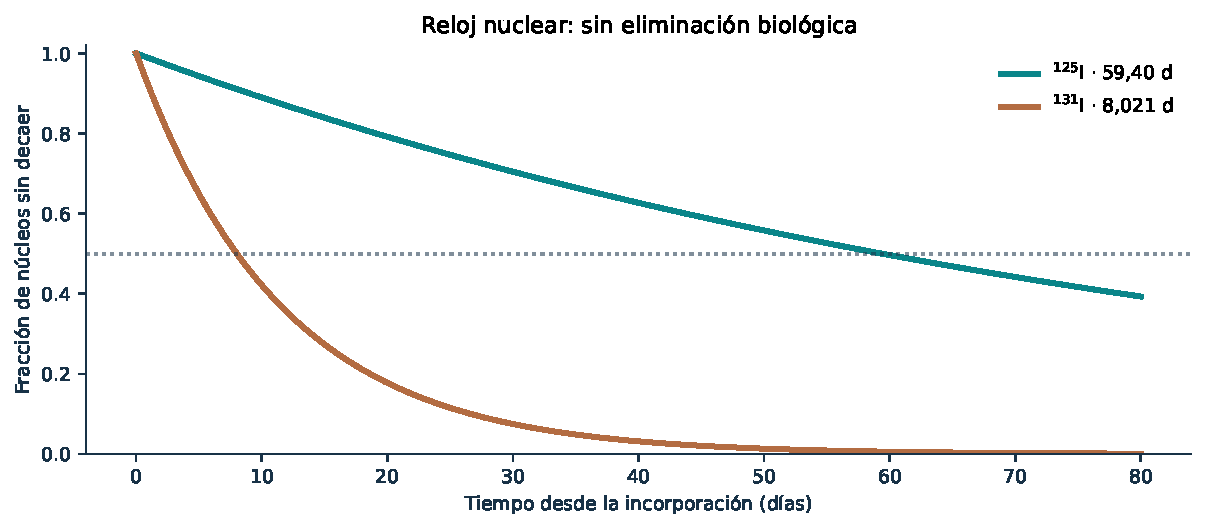
\includegraphics[width=.92\linewidth]{figuras_monografia/06_semividas_fisicas.pdf}
\caption{Supervivencia física de $^{125}$I y $^{131}$I calculada con las semividas
indicadas. No incorpora captación ni salida biológica.}\end{figure}

Con $T_{1/2}(^{125}\mathrm I)=59,40$ d y $t=18$ h $=0,75$ d,
$\lambda_{125}=0,011669$ d$^{-1}$ y
$F_{125}(0,75)=1-2^{-0,75/59,40}\simeq0,008714$.
Con $T_{1/2}(^{131}\mathrm I)=8,021$ d [7],
$\lambda_{131}=0,086416$ d$^{-1}$ y
$F_{131}(0,75)\simeq0,06275$. En idéntica ventana y para igual número
inicial de átomos, la fracción física que decae es mayor para $^{131}$I.
Ello no establece la dosis de una célula: los dos tipos de radiación y sus
geometrías de deposición difieren, y la cantidad incorporada podría ser distinta.

\clearpage
\subsection{Capítulo 9. Espectro beta de $^{131}$I y alcance de la aproximación}
\label{ampliacion-beta}

\subsubsection{Tres cuerpos y espectro continuo}
En el decaimiento beta menos, un neutrón se transforma en protón y se producen
un electrón y un antineutrino electrónico:
\begin{align}
n&\longrightarrow p+e^-+\bar\nu_e,\\
{}^{131}_{53}\mathrm I&\longrightarrow
 {}^{131}_{54}\mathrm{Xe}^{*}+e^-+\bar\nu_e.
\end{align}
La suma de energía cinética del electrón, del antineutrino y del retroceso,
más la excitación nuclear, iguala el valor $Q_\beta$. A diferencia de una
transición de dos cuerpos con masa hija fijada, el electrón y el antineutrino
comparten energía en una familia continua de configuraciones permitidas por
conservación de energía y momento. Si el núcleo hijo queda en distintos niveles,
cambia la energía final disponible para esa rama. Por ello \emph{un espectro de
una sola rama} no equivale al espectro total del $^{131}$I.

Para una rama permitida con endpoint $T_0$ y neutrino de masa despreciable,
una forma pedagógica de la densidad sin correcciones radiativas es
\begin{align}
\widetilde s(T)&=F(Z,T)\,p(T)\,[T+m_ec^2]\,(T_0-T)^2,\\
p(T)c&=\sqrt{T\big(T+2m_ec^2\big)},\qquad 0\leq T\leq T_0,\\
s(T)&=\frac{\widetilde s(T)}{\int_0^{T_0}\widetilde s(u)\,du},\qquad
C(T)=\int_0^T s(u)\,du.
\end{align}
El factor $(T_0-T)^2$ procede del espacio de fases aproximado del
antineutrino; $p(T)[T+m_ec^2]$ es la parte cinemática electrónica. La
función de Fermi $F(Z,T)$ corrige la interacción de Coulomb con el núcleo
hijo. En la figura se fija deliberadamente $F=1$ para mostrar solamente la
forma cinemática. El endpoint de 606,3 keV corresponde a una rama intensa
del $^{131}$I; no se debe confundir con la máxima energía de todas las ramas
ni con la energía media de sus electrones [15].

\begin{figure}[htbp]\centering
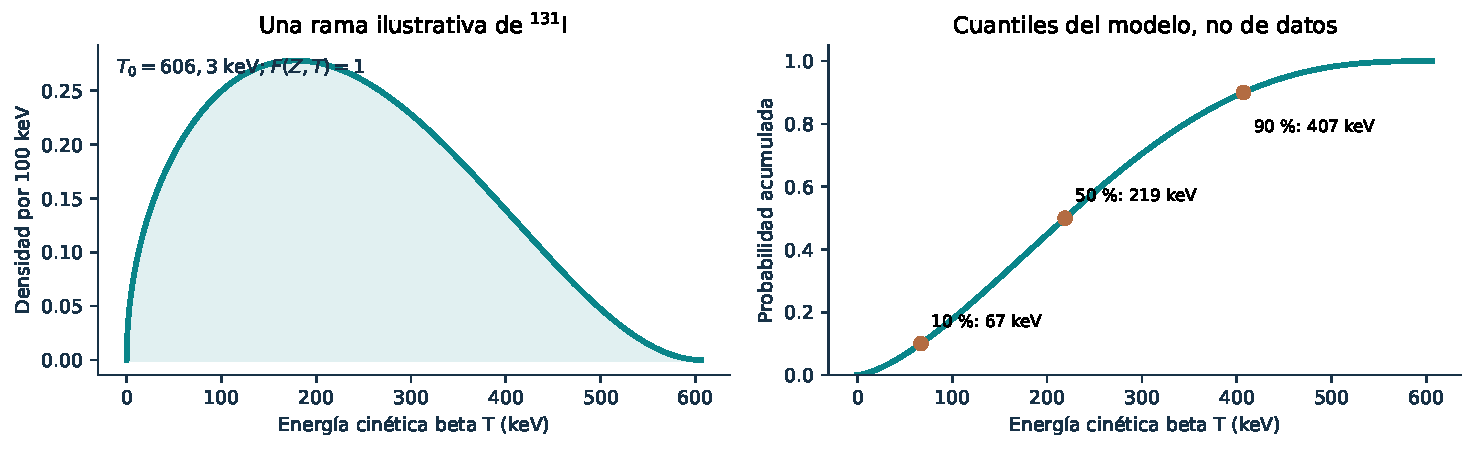
\includegraphics[width=.97\linewidth]{figuras_monografia/05_beta_modelo.pdf}
\caption{Espectro beta de una rama permitida y su distribución acumulada,
normalizados numéricamente con $T_0=606,3$ keV y $F=1$. Curvas derivadas,
no espectros medidos ni resultados de la simulación web.}\end{figure}

El área bajo $s(T)$ se fuerza a uno por integración trapezoidal. La CDF
comienza en cero y termina en uno por construcción. El cálculo arroja
cuantiles aproximados $T_{10}\simeq67$ keV,
$T_{50}\simeq219$ keV y $T_{90}\simeq407$ keV para \emph{este modelo}.
Cambiar la función de Fermi, la forma de transición, las ramas y sus
intensidades cambia esos valores. Su utilidad es conceptual: ni siquiera
una rama con endpoint fijo emite siempre electrones con la misma energía.
La gráfica no debe insertarse en una estimación de dosis de paciente como si
fuera una evaluación nuclear completa.

\subsubsection{Conservación y cinemática de un electrón de prueba}
La relación relativista entre energía total y momento es
\[
E^2=(pc)^2+(m_ec^2)^2,\qquad E=T+m_ec^2,\qquad
pc=\sqrt{T(T+2m_ec^2)}.
\]
Para $T=200$ keV y $m_ec^2=510,999$ keV,
\[
pc=\sqrt{200(200+2\cdot510,999)}\,\mathrm{keV}
\simeq494,37\,\mathrm{keV},
\qquad p\simeq494,37\,\mathrm{keV}/c.
\]
Ese número es el momento de \emph{un electrón supuesto} de 200 keV; no es
un momento representativo de todas las ramas. La presencia del antineutrino
es necesaria para el balance energético y leptónico. La emisión gamma desde
estados excitados de $^{131}$Xe pertenece a la desexcitación posterior y
tampoco se identifica con la energía del electrón beta.

\subsubsection{Relación con la escena interactiva}
La escena 01 de la web muestra captura y relajación para $^{125}$I; la escena
02 contrasta los dos relojes físicos y una salida hipotética. No hay una
escena que muestree el espectro beta de la figura: éste se incluye para
cubrir la física subatómica de $^{131}$I exigida por la monografía previa.
La escena 06 emplea una pendiente experimental de mutantes, sin obtenerla
por integración del espectro. No existe en el código una cadena de transporte
de partículas que conecte cada $T$ con un depósito energético local.

\clearpage
\subsection{Capítulo 10. Microdosimetría: volumen, distancia y definición de dosis}
\label{ampliacion-micro}

\subsubsection{De la energía a un promedio geométrico}
La dosis absorbida macroscópica es $D=d\bar\varepsilon/dm$, medida en
Gy $=\mathrm{J}/\mathrm{kg}$. Con un depósito supuesto $E_{\rm dep}$ uniforme
en una esfera acuosa de radio $r$ y densidad $\rho$, un promedio formal es
\begin{align}
V(r)&=\frac43\pi r^3,\\
m(r)&=\rho V(r),\\
D_{\rm esfera}(r)&=\frac{E_{\rm dep}}{\rho(4\pi r^3/3)}.
\end{align}
Si la energía y la densidad permanecen constantes, duplicar $r$ multiplica
el denominador por ocho y divide el promedio por ocho. Esto ilustra por qué
una energía pequeña puede corresponder a un cociente enorme si la masa
elegida es nanométrica. No significa que una desintegración deposite toda
su energía dentro de una esfera homogénea ni que ese cociente sea la dosis
celular medida.

Para reproducir el ejemplo del cuaderno de referencia, \emph{se supone}
$E_{\rm dep}=16,51$ keV y $r=10$ nm en agua de densidad
$\rho=1000\;\mathrm{kg,m^{-3}}$. Se convierten todas las unidades antes
de dividir:
\begin{align}
E_{\rm dep}&=16,51\times10^3\;\mathrm{eV}
  \times1,602176634\times10^{-19}\;\mathrm{J/eV}
  =2,64519\times10^{-15}\;\mathrm J,\\
r&=10\;\mathrm{nm}=10^{-8}\;\mathrm m,\\
V&=\frac43\pi(10^{-8}\;\mathrm m)^3
  =4,18879\times10^{-24}\;\mathrm{m^3},\\
m&=(1000\;\mathrm{kg/m^3})V
  =4,18879\times10^{-21}\;\mathrm{kg},\\
D_{\rm esfera}&=\frac{2,64519\times10^{-15}\;\mathrm J}
 {4,18879\times10^{-21}\;\mathrm{kg}}
  =6,315\times10^5\;\mathrm{Gy}.
\end{align}
La magnitud extrema procede \emph{del volumen escogido}, no de una dosis
medida en el núcleo o en el cuerpo. Si sólo la fracción $g$ de la energía
queda allí, el promedio sería $gD_{\rm esfera}$, con $0\leq g\leq1$;
en una traza real la distribución es heterogénea y no equivale a una esfera
uniforme. La figura permite inspeccionar el exponente $r^{-3}$.

\begin{figure}[htbp]\centering
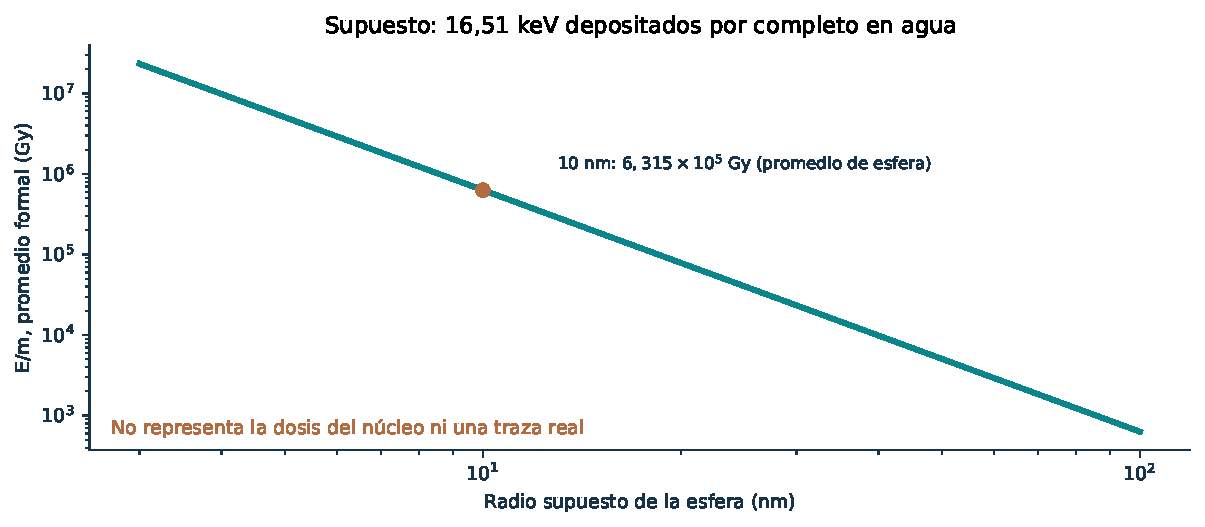
\includegraphics[width=.93\linewidth]{figuras_monografia/07_esfera_energia.pdf}
\caption{Cociente $E/m$ para una esfera de agua con energía supuestamente
depositada de 16,51 keV. El radio es una elección del ejemplo; el eje vertical
no representa dosimetría clínica ni una traza electrónica calculada.}\end{figure}

\subsubsection{Qué representa y qué no representa la distancia del modelo}
En la web, cada sitio $j$ de las dos hebras de una hélice B ideal de 60 pares
de bases tiene una posición $\mathbf x_j$. La fuente se coloca en
$\mathbf s$; se calcula $r_j=\|\mathbf x_j-\mathbf s\|$. Para parámetros
supuestos $\mu$ y $\ell$, la probabilidad de una oportunidad de lesión es
\[
p_j=1-\exp\!\left[-\mu\exp(-r_j/\ell)\right].
\]
Se puede derivar suponiendo que el número $K_j$ de oportunidades locales
es Poisson de media $\mu\exp(-r_j/\ell)$; entonces
$P(K_j\geq1)=1-P(K_j=0)=p_j$. El parámetro $\mu$ es adimensional y $\ell$
se mide en nm. El factor $\exp(-r_j/\ell)$ es una elección fenomenológica,
no una ley del frenado de electrones de Auger. El código toma sorteos
Bernoulli independientes por sitio; las correlaciones químicas verdaderas
quedan fuera de esta aproximación. El modelo de esfera de esta sección y el
modelo de Bernoulli del navegador son \emph{dos ilustraciones diferentes}:
no hay conversión en el programa de Gy por esfera a $\mu$ o $\ell$.

Una SSB operacional se marca cuando el sorteo en un sitio de una hebra
produce lesión. Una DSB operacional requiere dos marcas en hebras opuestas
cuya separación longitudinal en índices sea como máximo diez pares de bases.
Diez pares corresponden a unos $3,4$ nm a lo largo del eje de la hélice
ideal si se usa $0,34$ nm por par, pero la distancia tridimensional entre
sitios no es necesariamente $3,4$ nm. El número diez es una convención
del ejercicio, no un umbral biológico universal. El gráfico de sensibilidad
de la parte anterior muestra que variar $\mu$ y $\ell$ altera mucho las
frecuencias, razón por la cual no se interpretan como predicciones
experimentales de DSB por decaimiento [2].

\subsubsection{De microgeometría a una medición válida}
Una simulación de transporte defendible necesitaría el espectro de electrones
Auger y de conversión interna de cada rama, velocidades y direcciones,
colisiones inelásticas y elásticas, electrones secundarios, estado de
ionización de la molécula, agua y oxígeno, radicales, estructura molecular
del ADN y tiempos químicos. Después habría que definir lesiones,
compararlas con experimentos y propagar incertidumbres. Las gráficas de
este documento cumplen otra función: muestran cómo una \emph{hipótesis
espacial explícita} afecta un resultado, y permiten que otra persona
recalcule exactamente las mismas curvas con los archivos de código.

\clearpage
\subsection{Capítulo 11. De la actividad incorporada al número esperado de decaimientos}
\label{ampliacion-compartimentos}

\subsubsection{Contabilidad de actividad y fracciones}
Sean $A_0$ Bq administrados en un contexto hipotético, y $f_T,f_C,f_N,f_D$
las fracciones condicionales sucesivas que alcanzan tumor, célula, núcleo
y ADN. Un producto $f=f_Tf_Cf_Nf_D$ es una \emph{representación de
contabilidad} sólo si cada factor fue definido con el denominador correcto.
No se ha medido ninguno de ellos en el sitio web. El número de núcleos
iniciales asociados a ADN se escribiría
\[
N_{D,0}=f\frac{A_0}{\lambda},
\qquad [A_0]=\mathrm{s^{-1}},\quad[\lambda]=\mathrm{s^{-1}}.
\]
No hay que confundir $f$ con la probabilidad de mutación $f_{\rm HPRT}$.
Si la actividad se mide después de la incorporación, se usa la actividad
de ese compartimento y no se multiplica otra vez por las fracciones de
captación. Esta aclaración evita contar la incorporación dos veces.

\subsubsection{Dos riesgos competitivos y su derivación}
Sea $\lambda$ la tasa nuclear y $k$ una tasa de salida del compartimento
ADN, ambas constantes en el ejemplo. La probabilidad de que un núcleo
continúe allí y sin decaer hasta $t$ satisface
\begin{align}
S_D(t)&=\exp[-(\lambda+k)t],\\
P_{\rm dec\,en\,ADN}(t)
 &=\int_0^t\lambda S_D(u)\,du
 =\frac{\lambda}{\lambda+k}
    \bigl(1-e^{-(\lambda+k)t}\bigr),\\
P_{\rm sale}(t)
 &=\frac{k}{\lambda+k}
    \bigl(1-e^{-(\lambda+k)t}\bigr).
\end{align}
La suma $P_{\rm dec\,en\,ADN}(t)+P_{\rm sale}(t)+S_D(t)=1$ es una
prueba de conservación. A tiempos largos, la fracción que decae antes de
salir es $\lambda/(\lambda+k)$. Si $k=0$, tiende a uno; si
$k\gg\lambda$, tiende a cero. La \emph{semivida efectiva} de la población
que permanece en el compartimento es $T_{1/2,\rm ef}=\ln2/(\lambda+k)$.
Esto no reemplaza la semivida nuclear: una molécula que sale sigue
conteniendo un radionúclido con la misma tasa de desintegración, pero ya
no decae en la ubicación modelada.

\begin{figure}[htbp]\centering
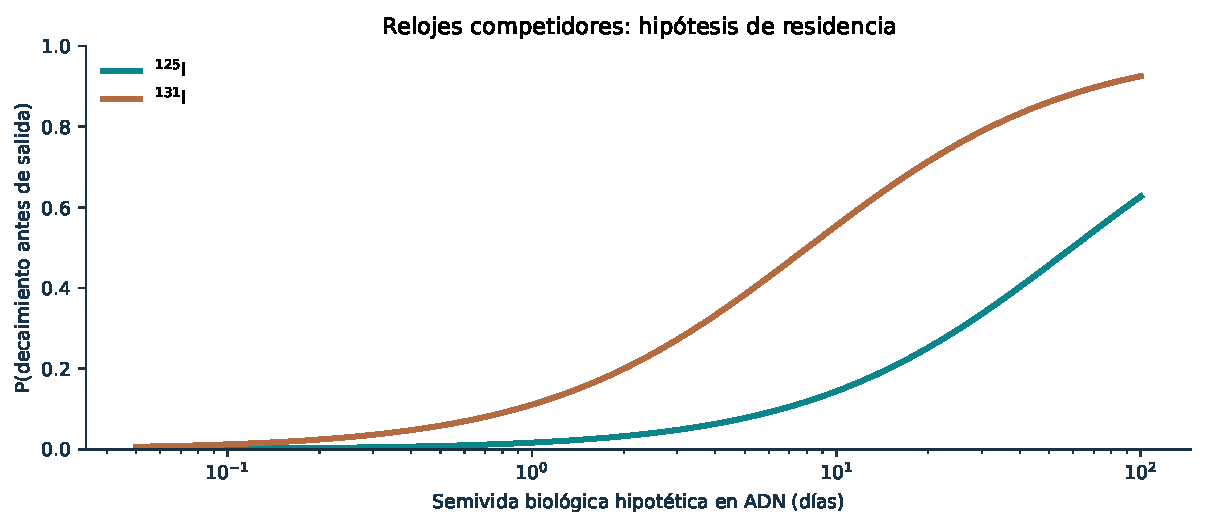
\includegraphics[width=.92\linewidth]{figuras_monografia/08_competencia_biologica.pdf}
\caption{Probabilidad límite de decaer antes de abandonar ADN frente a una
semivida biológica elegida. La curva es una consecuencia del modelo de riesgos
competitivos; no mide retención en TK6 ni biocinética humana.}\end{figure}

La escena 02 implementa precisamente esta competencia. Si el usuario mueve
el deslizador de salida, modifica $k$ y ve un resultado condicional del
modelo. La figura no permite seleccionar una dosis prescrita ni conocer
retención real. En un paciente $k$ podría variar con el tiempo, la célula,
la división y el metabolismo; haría falta un modelo biocinético validado
para remplazar la constante hipotética.

\subsubsection{Propagación de una incertidumbre elemental}
Para $P_\infty=\lambda/(\lambda+k)$,
\[
\frac{\partial P_\infty}{\partial k}
 =-\frac{\lambda}{(\lambda+k)^2},\qquad
\frac{\partial P_\infty}{\partial\lambda}
 =\frac{k}{(\lambda+k)^2}.
\]
Si $k$ se incrementa, la probabilidad disminuye; si $\lambda$ aumenta
manteniendo $k$, aumenta. Bajo errores pequeños e independientes, una
propagación lineal sería
\[
\sigma_P^2\simeq
 \left(\frac{\partial P}{\partial\lambda}\sigma_\lambda\right)^2+
 \left(\frac{\partial P}{\partial k}\sigma_k\right)^2.
\]
El texto no da un valor numérico de $\sigma_k$, porque no hay medición de
retención en el proyecto. Fijar arbitrariamente uno haría parecer calibrado
un ejemplo que no lo está. El error estándar binomial reportado por la
escena de DSB, por su parte, cuantifica sólo variación del muestreo con
parámetros fijos, no esta incertidumbre de modelo.

\clearpage
\subsection{Capítulo 12. Resultados externos en material humano}
\label{ampliacion-evidencia}

\subsubsection{Linfocitos y la importancia de leer el corrigendum}
El estudio de Schmitz y colaboradores expuso linfocitos humanos de sangre
periférica al $^{125}$I--UdR y examinó aberraciones cromatídicas y muerte
celular [12]. Su población marcada era heterogénea: el resumen público
describe cerca de 40\% de células muy marcadas, 20\% moderadamente
marcadas y 40\% sin marcar. Un promedio de actividad puede por tanto
ocultar exposiciones muy diferentes dentro del mismo cultivo. La
publicación de 2016 corrigió expresamente una inferencia numérica de la
versión de 2015: con nueve experimentos, sus datos indicaron \emph{en
promedio unas 250 desintegraciones por aberración cromosómica} en las
condiciones medidas [9]. Así, un ejemplo aritmético de 2500
desintegraciones produciría una esperanza de 10 aberraciones bajo una
extrapolación lineal del cociente, \emph{no} diez DSB observadas y tampoco
diez mutaciones HPRT. La heterogeneidad celular y la selección de
metafases limitan la traslación directa. Se cita la corrección junto al
artículo original para no repetir la interpretación retractada.

\subsubsection{Biodistribución y localización en pacientes}
Mariani y colaboradores estudiaron diez personas con cáncer colorrectal
después de una inyección intratumoral de $^{125}$I--UdR de 0,24 a
3,9 MBq antes de cirugía [13]. Midieron actividad en tumor y tejidos
vecinos y usaron microautoradiografía de cortes resecados. El resumen
publicado informa que esta última mostró localización en núcleos de
células tumorales humanas. Esto responde una pregunta distinta a la del
ensayo HPRT: confirma que la molécula puede alcanzar la ubicación
celular relevante bajo esa vía concreta, pero no mide con ello una tasa
de mutación en un paciente. Además, la distribución intratumoral y la
incorporación normal no son homogéneas por definición. La cifra media
de actividad por gramo y la relación tumor/tejido vecino del artículo
no deben tratarse como fracciones universales del modelo de la web.

\subsubsection{Primer caso terapéutico y límites de inferencia}
Rebischung y colaboradores publicaron en 2008 una primera experiencia
humana de administración intratecal de $^{125}$I--UdR junto con
metotrexato para meningitis neoplásica resistente [14]. Un caso permite
discutir factibilidad, seguimiento y preguntas de seguridad; no permite
aislar el efecto del radiofármaco respecto al metotrexato ni estimar
eficacia general. En esta monografía sirve de puente entre un mecanismo
en cultivo y el tipo de problemas que aparecen en seres humanos. No se
infieren de él indicaciones, dosis clínicas, probabilidad personal de
mutación o beneficio terapéutico. El foco experimental cuantitativo
continúa siendo Whaley y Little [1].

\begin{table}[htbp]\centering\small
\begin{tabularx}{\linewidth}{@{}p{.19\linewidth}p{.31\linewidth}X@{}}
\toprule Fuente & Observación pertinente & Inferencia autorizada \\\midrule
Whaley y Little [1] & Mutantes HPRT y supervivencia, TK6/SE30 & Eficacia relativa de decaimientos incorporados en células humanas bajo el ensayo. \\
Schmitz et al. [12,9] & Aberraciones en linfocitos y corrección de 250 desintegraciones por aberración & Un endpoint citogenético y su cifra corregida, no DSB por desintegración. \\
Mariani et al. [13] & Microautoradiografía tras inyección en diez pacientes & Localización nuclear tumoral bajo una ruta específica, no tasa clínica de mutaciones. \\
Rebischung et al. [14] & Primer caso intratecal con tratamiento combinado & Factibilidad y preguntas clínicas; no eficacia general ni atribución aislada. \\\bottomrule
\end{tabularx}
\caption{Cuatro niveles de evidencia que no se convierten unos en otros por una sola ecuación.}
\end{table}

La figura de la escena 06 representa de manera pedagógica una pendiente de
mutantes publicada [1]. La escena 04 produce una frecuencia de DSB
\emph{simulada} a partir de probabilidades supuestas. Nunca se ajustó
$\mu$ hasta que la frecuencia de DSB coincidiera con los 250 decaimientos
por aberración de un experimento distinto. Hacerlo sin un modelo de
reparación y observación de cromosomas equivaldría a identificar endpoints
incompatibles.

\clearpage
\subsection{Capítulo 13. Cálculos resueltos y comprobaciones dimensionales}
\label{ampliacion-ejercicios}

\subsubsection{Problema 1: un intervalo de dieciocho horas}
Se pregunta qué fracción de un conjunto de $N_0$ átomos \emph{incorporados y
retenidos por hipótesis} decae en dieciocho horas. Primero se expresa el
tiempo en la misma unidad de la semivida: $18\,\mathrm h=18/24=0,75$ d.
Después se calcula $\lambda=\ln2/T_{1/2}$, con dimensión d$^{-1}$.
Finalmente se evalúa $1-\exp(-\lambda t)$. Usando $59,40$ y $8,021$ d,
respectivamente, se obtiene
\begin{align}
\lambda_{125}&=\frac{0,693147}{59,40\;\mathrm d}
  \simeq0,0116691\;\mathrm d^{-1},\\
F_{125}(18\,\mathrm h)&=1-e^{-0,0116691(0,75)}
  \simeq0,008714\simeq0,8714\%,\\
\lambda_{131}&=\frac{0,693147}{8,021\;\mathrm d}
  \simeq0,086416\;\mathrm d^{-1},\\
F_{131}(18\,\mathrm h)&=1-e^{-0,086416(0,75)}
  \simeq0,06275\simeq6,275\%.
\end{align}
Cada exponente es adimensional. El resultado $F_{131}/F_{125}\simeq7,20$
compara \emph{fracciones de átomos iniciales} que decaen, no dosis,
mutaciones ni actividades administradas. Si se usara una semivida tabulada
de $8,0252$ d como en el cuaderno anterior, habría una diferencia pequeña
en las últimas cifras; aquí se mantiene $8,021$ d de ICRP [7] para coincidir
con el programa. Una semivida biológica distinta modificaría el número de
decaimientos que tienen lugar antes de salir del ADN.

\subsubsection{Problema 2: convertir una actividad en núcleos}
Supóngase una actividad inicial de $A_0=1000$ Bq de $^{125}$I en un
compartimento \emph{hipotético}. Una actividad de 1000 Bq significa
1000 desintegraciones esperadas por segundo en ese instante. Convertimos
la constante nuclear:
\begin{align}
T_{1/2}&=59,40\;\mathrm d\times86400\;\mathrm{s/d}
  =5\,132\,160\;\mathrm s,\\
\lambda&=\frac{0,693147}{5\,132\,160\;\mathrm s}
  \simeq1,3506\times10^{-7}\;\mathrm{s^{-1}},\\
N_0&=\frac{A_0}{\lambda}
  \simeq\frac{1000\;\mathrm{s^{-1}}}{1,3506\times10^{-7}\;\mathrm{s^{-1}}}
  \simeq7,40\times10^9\;\text{núcleos}.
\end{align}
Este número no dice cuántos átomos están en ADN: para ello habría que medir
la actividad de esa fracción o introducir una fracción de incorporación
con incertidumbre. La igualdad $A=\lambda N$ relaciona una esperanza
instantánea con la cantidad de átomos, no una cuenta exacta de eventos
individuales en un intervalo corto.

\subsubsection{Problema 3: pendiente HPRT y cambio de unidades}
La pendiente experimental de $^{131}$I--IdUrd en TK6 se reporta como
$\alpha=0,45\times10^{-6}\,\mathrm{cGy}^{-1}$ de mutantes inducidos por
célula clonable [1]. Como $1\,\mathrm{Gy}=100\,\mathrm{cGy}$, el mismo
producto $\alpha D$ debe mantenerse al cambiar de unidad:
\[
\alpha=45\times10^{-6}\,\mathrm{Gy}^{-1}.
\]
Si se \emph{extiende linealmente} la pendiente hasta $D=38$ cGy
$=0,38$ Gy,
\begin{align}
\Delta f&=(0,45\times10^{-6}\,\mathrm{cGy}^{-1})
                 (38\,\mathrm{cGy})\\
 &=17,1\times10^{-6}
 =17,1\;\text{mutantes inducidos por millón de células clonables}.
\end{align}
El mismo resultado surge de $(45\times10^{-6}\,\mathrm{Gy}^{-1})(0,38\,
\mathrm{Gy})$. Los 38 cGy en el resumen del artículo describen el límite
de dosis mencionado para \emph{SE30} con decaimientos en el medio; no
constituyen una medida directa de TK6 a ese punto. Así, $17,1$ es una
extrapolación aritmética expresamente rotulada, no una observación [1].

\subsubsection{Problema 4: del valor esperado al conteo de pocillos}
Si $n$ células clonables por pocillo tienen frecuencia efectiva
$f(D)=f_0+\alpha D$ y se aceptan los supuestos de rareza e independencia,
$Y\sim\mathrm{Poisson}(nf(D))$. Para $m$ pocillos independientes,
la suma $Y_\mathrm{total}$ sería Poisson de media $mnf(D)$.
Si una población sólo tiene $n=1000$ células clonables por pocillo,
$f_0=10\times10^{-6}$ es un fondo \emph{elegido} y se usa
$D=38$ cGy como ejemplo aritmético, entonces
\[
f(D)=27,1\times10^{-6},\quad
E[Y]=0,0271,\quad P(Y=0)=e^{-0,0271}\simeq0,9733.
\]
Es posible que la mayoría de pocillos no tenga mutantes resistentes
incluso con una frecuencia inducida distinta de cero. Variar el número
de pocillos cambia la precisión estadística, no la frecuencia biológica.
En la aplicación el fondo, el número de células y el generador aleatorio
son controles del escenario, no valores medidos por Whaley y Little.

\subsubsection{Problema 5: un intervalo de incertidumbre del Monte Carlo}
Si $n_\mathrm{sim}$ desintegraciones simuladas generan $k$ sucesos DSB,
$\widehat p=k/n_\mathrm{sim}$ y el error estándar binomial aproximado es
\[
\operatorname{SE}(\widehat p)=
\sqrt{\frac{\widehat p(1-\widehat p)}{n_\mathrm{sim}}}.
\]
Por ejemplo, si $k=350$ entre $n_\mathrm{sim}=3500$ corridas,
$\widehat p=0,10$ y $\mathrm{SE}\simeq0,00507$.
Una banda normal aproximada al 95\% sería $0,10\pm1,96(0,00507)$,
es decir aproximadamente $[0,0901;0,1099]$. Cerca de cero, una banda
normal simétrica puede funcionar mal; es preferible Wilson o un método
binomial exacto. Ninguno de estos intervalos cubre el error por un perfil
espacial equivocado o por omitir procesos químicos.

\subsubsection{Problema 6: integrar tres destinos competidores}
Sea $L(t)$ la probabilidad de una lesión inicial aún sin resolución,
con tasas $k_r,k_m,k_p$ de reparación, fijación de mutación y pérdida
celular. Si $L(0)=1$ y $R(0)=M(0)=C(0)=0$,
\begin{align}
\dot L&=-(k_r+k_m+k_p)L,&
\dot R&=k_rL,&\dot M&=k_mL,&\dot C&=k_pL.
\end{align}
Para $K=k_r+k_m+k_p$,
\begin{align}
L(t)&=e^{-Kt},\\
R(t)&=\frac{k_r}{K}(1-e^{-Kt}),\\
M(t)&=\frac{k_m}{K}(1-e^{-Kt}),\\
C(t)&=\frac{k_p}{K}(1-e^{-Kt}).
\end{align}
La suma es uno para todo $t$ y cada término permanece entre cero y uno
cuando las tasas son no negativas. Un control en JavaScript y Python prueba
esta identidad para los parámetros del ejercicio. Las categorías son
estados \emph{conceptuales} del modelo; una célula real puede contener
múltiples lesiones y experimentar procesos más complejos. En particular,
$M(t)$ no equivale a frecuencia HPRT medida, porque aún faltan supervivencia,
expresión y selección.

\clearpage
\subsection{Capítulo 14. Reproducibilidad exacta del atlas actual}
\label{ampliacion-software}

\subsubsection{Seis escenas y sus variables reales}
La monografía de referencia de septiembre describía una propuesta de siete
módulos, incluido un espectro beta y un recorrido de paciente a ADN. El
repositorio terminado en noviembre contiene \emph{seis} escenas distintas.
Esta correspondencia actualizada evita presentar una funcionalidad antigua
como si estuviera implementada:
\begin{table}[htbp]\centering\footnotesize
\begin{tabularx}{\linewidth}{@{}p{.19\linewidth}p{.35\linewidth}X@{}}
\toprule Página del atlas & Entrada y cálculo & Lectura correcta \\\midrule
01 Captura y Auger & Animación Canvas de transformación y relajación & Esquema explicativo; no transporte ni espectro Auger calculado. \\
02 Semividas y retención & $N/N_0$, actividad y riesgos $\lambda,k$ & Semividas tabuladas; salida biológica supuesta. \\
03 Distancia al ADN & Geometría B ideal, $r_j$, $p_j(\mu,\ell)$ & Perfil fenomenológico, no alcance de electrones medido. \\
04 Roturas agrupadas & Bernoulli por sitio y criterio de 10 pb & Frecuencia Monte Carlo de DSB operacional. \\
05 Reparación y mutación & $L,R,M,C$ por tres tasas elegidas & Destinos competidores ilustrativos, no mediciones de reparación. \\
06 Ensayo HPRT & Pendiente publicada, fondo elegido, Poisson & Un dato TK6 de [1] y extrapolaciones marcadas. \\\bottomrule
\end{tabularx}
\caption{Mapa de la implementación revisada; las escenas 04 y 06 forman la exposición principal.}
\end{table}

El núcleo \path{science.js} calcula magnitudes compartidas y administra
el estado físico de las escenas. \path{lab.js} crea controles, dibuja los
Canvas y muestra salidas; los archivos HTML enlazan cada laboratorio.
\path{python/modelo.py} reproduce una cadena de cálculos con NumPy y
genera un resumen JSON; \path{python/verificar.py} contiene cinco
comprobaciones físicas y matemáticas. El navegador y NumPy no usan el
mismo generador pseudoaleatorio: coincidencia de ecuaciones y de
distribuciones no implica igualdad de cada realización aleatoria.

\subsubsection{Correspondencia de ecuaciones, código y pruebas}
La variable $\lambda$ se construye a partir de la semivida, y la actividad
disminuye como $\lambda N(t)$. El límite temporal y la conservación se
prueban con $N(T_{1/2})=N_0/2$ y
$P_{\rm dec}+P_{\rm sale}+S_D=1$. La geometría usa distancias
tridimensionales del eje y de las dos hebras, y el algoritmo distingue
una separación de diez pares de una de once. La conservación
$L+R+M+C=1$ se verifica para los destinos. La pendiente HPRT se prueba
en unidades cGy y Gy. La simulación Monte Carlo se repite con semilla
fija; un control analítico independiente compara la frecuencia de
\emph{alguna} rotura bajo la hipótesis de independencia,
\[
P(\text{alguna rotura})=1-\prod_{j}(1-p_j).
\]
La DSB, que requiere marcas en hebras opuestas, no se obtiene de esta
última fórmula simple; se contabiliza en la muestra y se somete a una
prueba separada con casos de borde. El anexo imprime los archivos
ejecutados, no fragmentos reescritos para la monografía.

Para reconstruir desde la raíz del repositorio se instalan las
dependencias declaradas, se genera el resumen y se ejecutan pruebas:
\begin{verbatim}
python -m pip install -r python/requirements.txt
python python/modelo.py
python python/verificar.py
node --test tests/science.test.mjs
python tests/check_links.py
\end{verbatim}
Los cuatro gráficos de los primeros capítulos se generan con
\path{python/crear_monografia_final.py}; los cuatro gráficos vectoriales
de esta ampliación provienen de \path{python/figuras_ampliacion.py}.
Los archivos PDF de figuras se incluyen como vectores en XeLaTeX.
Para reproducir las animaciones MP4 existe \path{python/animar.py}; su
ejecución requiere FFmpeg, y los vídeos entregados ya están incluidos
en el sitio. La reproducción de las pruebas no constituye validación
experimental del perfil espacial ni de tasas biológicas supuestas.

\subsubsection{Trazabilidad y revisión de cifras}
Los valores de semivida, modo de decaimiento y línea gamma se atribuyen
a tablas de IAEA e ICRP [6--8]. El endpoint beta de 606,3 keV procede
de la rama descrita en una fuente nuclear [15]; su curva $F=1$ es
\emph{nuestra} aproximación. La pendiente HPRT pertenece a [1]; $17,1$
por millón a 38 cGy se obtiene multiplicando, con una advertencia
expresa sobre los distintos grupos. La cifra de unas 250
desintegraciones por aberración está en el corrigendum [9], no en una
predicción de nuestro Monte Carlo. Los parámetros $\mu$, $\ell$, $k$,
$k_r$, $k_m$, $k_p$ y $f_0$ son elecciones visibles en controles o
documentadas en el código. Una tabla de procedencia permite verificar
qué se puede y qué no se puede reclamar ante el curso.

\begin{table}[htbp]\centering\footnotesize
\begin{tabularx}{\linewidth}{@{}p{.24\linewidth}p{.31\linewidth}X@{}}
\toprule Magnitud & Procedencia & Estatus epistemológico \\\midrule
59,40 d; 8,021 d & ICRP [7] & Datos físicos tabulados. \\
35,49 keV; 6,68\% & IAEA [6] & Línea y probabilidad de transición nuclear. \\
606,3 keV & IAEA [15] & Endpoint de una rama beta, no energía constante. \\
$0,45\times10^{-6}$/cGy & Whaley y Little [1] & Pendiente de mutantes HPRT en TK6 para $^{131}$I--IdUrd. \\
250 decaimientos por aberración & Schmitz et al., corrección [9] & Promedio experimental de otro endpoint y condiciones. \\
$\mu,\ell,k$ y tasas de destino & Configuración del programa & Hipótesis ilustrativas sin ajuste experimental. \\
16,51 keV en esfera & Ejercicio de cuaderno & Energía supuesta con depósito completo, no dosimetría real. \\\bottomrule
\end{tabularx}
\caption{Procedencia y límites de las cifras centrales de la monografía.}
\end{table}

\clearpage
\subsection{Capítulo 15. Correspondencia con Física Subatómica y análisis de sensibilidad}
\label{ampliacion-programa}

\subsubsection{Del nucleón al leptón: qué enseña la comparación isotópica}
El problema comienza con dos transformaciones débiles cargadas diferentes.
En captura electrónica se destruye un electrón ligado y se crea un
neutrino electrónico; en beta menos se crea un electrón y un
antineutrino. En ambos casos se conserva la carga y el número leptónico
con la convención apropiada. El nucleón cambia su identidad mientras
el número másico del núcleo permanece constante. Para $^{125}$I se
reduce $Z$ de 53 a 52, y para $^{131}$I aumenta de 53 a 54. Esa
contabilidad conecta las bases del curso con los dos mecanismos que
puede contrastar el público. El estado nuclear hijo puede estar excitado:
la desexcitación es otra etapa física y no debe mezclarse con el vértice
débil. Tampoco la conversión interna, una transferencia de energía de
una transición nuclear a un electrón orbital, es sinónimo de captura
electrónica, que transforma un protón.

La conservación del cuadrimomento explica por qué los términos de
energía son necesarios. En una rama beta $Q_\beta$ debe distribuirse
entre dos partículas ligeras y un retroceso, además de cualquier
excitación de la hija. En captura electrónica el neutrino transporta
una parte sustancial de la energía de cada canal y el átomo queda con
una vacante; resolver una igualdad de $Q$ no significa conocer cada
emisión final. El diagrama de Feynman que esquematiza la interacción
débil a nivel de quarks representa amplitudes y líneas de partículas,
no trayectorias espaciales de electrones Auger dentro de una hélice.
Esta separación es útil para defender oralmente el proyecto: un dibujo
de una partícula saliendo del átomo es una guía conceptual, mientras
una gráfica de energía requiere datos de niveles y ramificaciones.

La forma beta permitida del capítulo 9 utiliza la cinemática relativista
del electrón, el espacio de fases del antineutrino y un factor de Coulomb
que allí se fijó en uno. La palabra \emph{permitida} tiene un contenido
de selección nuclear y forma espectral: una transición con distinta
estructura puede exigir otros factores. Por eso la curva es un ejercicio
de curso bien delimitado, no una evaluación precisa de todas las ramas
de $^{131}$I. Las diapositivas de decaimientos aportadas al proyecto
[10] motivan la conservación de carga, energía y número leptónico; la
literatura nuclear proporciona los valores tabulados [6--8,15].

\subsubsection{Qué detecta un instrumento y qué selecciona un cultivo}
Los detectores de radiación responden a interacciones de partículas o
fotones con un material: una señal eléctrica o luminosa puede permitir
inferir energía depositada o contar eventos según la configuración del
instrumento [11]. Un detector no informa por sí mismo que una célula
ha fijado una mutación. El ensayo HPRT invierte la lógica: cultiva
células, aplica selección y cuenta descendencia resistente después
de un proceso biológico. En medio hay una cadena de hechos que no
puede reducirse a la lectura de un dosímetro. Incluso la dosis absorbida
por un núcleo celular es una energía media sobre masa, mientras la
disposición de ionizaciones individuales en nanómetros determina
correlaciones que esa media no registra. Esta relación entre señal
física y endpoint biológico explica por qué se necesitan tanto las
escenas de mecanismos como las dos escenas de exposición elegidas.

En la representación visual se emplean colores y movimientos para
separar categorías: radiación emitida, geometría de dos hebras,
lesiones, destinos y colonias. La flecha entre categorías es una
hipótesis causal, no una observación cuadro a cuadro de un mismo
experimento. El vídeo de roturas muestra un criterio de diez pares;
la interfaz HPRT muestra mutantes por millón de células clonables.
La unidad del primer resultado es una fracción de \emph{corridas de
Monte Carlo}; la del segundo es una frecuencia fenotípica y una
pendiente por cGy obtenida en TK6. No se convierten con un simple
factor de escala. Para establecer un puente cuantitativo harían falta
una respuesta de reparación y supervivencia medida en la misma
población, además de calibrar el transporte de energía.

\subsubsection{Derivadas del perfil espacial: qué hace cada deslizador}
La función elegida para la oportunidad local es
$p(r,\mu,\ell)=1-\exp[-\mu\exp(-r/\ell)]$.
Definamos $a=\mu e^{-r/\ell}$; entonces $p=1-e^{-a}$.
Derivando paso a paso a distancia y escala fijas,
\begin{align}
\frac{\partial a}{\partial\mu}&=e^{-r/\ell},&
\frac{\partial p}{\partial\mu}
 &=e^{-a}e^{-r/\ell}>0.
\end{align}
Aumentar $\mu$ nunca disminuye la probabilidad por sitio. En cambio,
derivando respecto a la distancia,
\begin{align}
\frac{\partial a}{\partial r}&=-\frac{a}{\ell},&
\frac{\partial p}{\partial r}&=-\frac{a}{\ell}e^{-a}<0
\quad(\ell>0).
\end{align}
Así, alejar \emph{ese sitio} de la fuente reduce su probabilidad.
La interfaz mueve una fuente completa frente a una geometría 3D;
algunos sitios pueden cambiar su distancia de forma distinta, por lo
que el argumento de derivada individual no debe sustituir la
inspección de todos los $r_j$. Para la escala,
\[
\frac{\partial p}{\partial\ell}
=e^{-a}\,a\frac{r}{\ell^2}\geq0
\quad(r\geq0),
\]
lo cual muestra por qué un perfil más ancho aumenta las oportunidades
en sitios a distancia no nula dentro de \emph{este modelo}.
Ninguna de estas derivadas determina la sensibilidad de una célula
real si $\mu$ y $\ell$ no han sido medidos.

El evento \emph{alguna rotura} bajo independencia tiene probabilidad
$1-\prod_j(1-p_j)$ y crece si crece cualquiera de los $p_j$.
La DSB del algoritmo es un evento compuesto: exige una pareja
compatible en hebras opuestas. Puede aumentar con los mismos
parámetros, pero su magnitud y la forma de la curva dependen de la
posición de la fuente, la geometría y la ventana de diez pares.
El error estándar del Monte Carlo se reduce aproximadamente como
$n_{\rm sim}^{-1/2}$ al aumentar las corridas; el sesgo por el
perfil espacial elegido no desaparece así. Si la incertidumbre del
muestreo es pequeña y la variación de parámetros domina, añadir
millones de corridas no resolverá la pregunta física principal.

\subsubsection{Por qué una monografía requiere referencias y reproducibilidad}
Una cifra puede ser correcta aritméticamente y, sin embargo, estar
asignada al endpoint equivocado. El ejemplo de $17,1$ se calcula
sin dificultad, pero debe identificarse como extensión lineal de la
pendiente TK6 a un valor de dosis citado para el contexto SE30.
La corrección de Schmitz muestra el riesgo más severo: una frase
cuantitativa de una publicación inicial fue rectificada y no debe
seguirse reproduciendo como tasa de aberraciones [9,12]. La
trazabilidad exige un registro de fuente, fecha, población, unidad,
condición y significado de cada número. Las funciones de prueba del
repositorio cubren identidades de ecuaciones y casos extremos; la
lectura crítica de artículos cubre algo diferente, la correspondencia
entre una afirmación y el experimento del que procede. Ambos controles
son necesarios para presentar con honestidad un trabajo que junta
física nuclear, biología y software.

\clearpage
\subsection{Capítulo 16. Límites, síntesis y respuesta a la pregunta}
\label{ampliacion-conclusiones}

La pregunta rectora es si la incorporación de un radionúclido al ADN humano
modifica la respuesta biológica y cómo explicarla desde física subatómica.
El artículo conductor respalda una respuesta afirmativa \emph{para sus
condiciones de cultivo}: TK6 incorpora mejor el análogo; cuando
$^{125}$I o $^{131}$I decaen desde esa localización, los efectos de
muerte y mutación son mayores que con actividad no incorporada [1].
La física explica por qué la ubicación importa: la transformación
nuclear fija qué partículas se emiten; la relajación atómica del $^{125}$I
origina electrones de baja energía; el beta de $^{131}$I nace con un
espectro continuo y en el ADN cambia el origen de su traza. Sin embargo,
ninguna de estas identidades nucleares, por sí sola, determina cuántos
mutantes fijados aparecerán: median geometría, química, reparación,
supervivencia y selección.

La simulación del repositorio cumple una función bien acotada. La escena
04 hace visible cómo distancia, oportunidad de lesión y criterio de dos
hebras producen una frecuencia \emph{bajo un modelo}. La escena 06 conecta
un resultado HPRT publicado con conversión de unidades, extrapolación
lineal y variabilidad de conteos. Esas dos escenas, elegidas para la
exposición, permiten contar el recorrido biológico desde la lesión hasta
un ensayo de mutación, mientras las otras cuatro aportan el fundamento
físico y el contexto. El atlas, las gráficas y el anexo pueden reproducirse
con el código; ni la coincidencia entre implementaciones ni la estética
de la animación convierten parámetros libres en constantes de la naturaleza.

La monografía de referencia aportada por los autores dedicaba capítulos
a espectro beta, esfera nanométrica, evidencia en linfocitos y pacientes.
Aquí esas materias se conservan como \emph{desarrollo ampliado} y se
relacionan con la implementación terminada. Se respetan cuatro fronteras:
\begin{enumerate}[leftmargin=*,itemsep=2pt]
\item un cociente de energía y masa en una esfera supuesta no es una dosis
      humana medida;
\item una DSB operacional simulada no es una aberración citogenética ni una
      mutación HPRT observada;
\item la pendiente de TK6 no se convierte directamente en riesgo individual
      o en frecuencia de todo el genoma;
\item una serie clínica pequeña o un caso combinado no establecen eficacia
      terapéutica general.
\end{enumerate}

Un siguiente estudio cuantitativo requeriría medir incorporación y
retención en ADN de cada población, utilizar datos de emisiones por rama,
modelar transporte y química a nanoescala, comparar lesiones con ensayos
independientes y ajustar la cinética de reparación a mediciones. En el
proyecto actual, las preguntas que sí se pueden contestar sin esos datos
son más precisas: qué ecuaciones gobiernan la desintegración, qué
predicción se sigue de cada supuesto, qué magnitud se midió realmente y
qué resultado de la simulación cambia al mover un parámetro. Esa
separación hace que el trabajo sea reproducible y defendible ante una
exposición de Física Subatómica.

\section{Referencias}\label{referencias}

\begin{enumerate}
\def\labelenumi{\arabic{enumi}.}
\tightlist
\item
  Whaley, J. M. y Little, J. B. (1990). ``Efficient mutation induction by 125I and 131I decays in DNA of human cells''. \emph{Radiation Research} \textbf{123}(1), 68--74. \href{https://pubmed.ncbi.nlm.nih.gov/2371380/}{PMID 2371380}; \href{https://doi.org/10.2307/3577659}{DOI 10.2307/3577659}. Los datos numéricos atribuidos se cotejaron con el resumen público; el texto íntegro puede requerir acceso institucional.
\item
  Martin, R. F. y Haseltine, W. A. (1981). ``Range of radiochemical damage to DNA with decay of iodine-125''. \emph{Science} \textbf{213}, 896--898. \href{https://pubmed.ncbi.nlm.nih.gov/7256283/}{PMID 7256283}; \href{https://doi.org/10.1126/science.7256283}{DOI 10.1126/science.7256283}.
\item
  LeMotte, P. K. y Little, J. B. (1984). ``DNA damage induced in human diploid cells by decay of incorporated radionuclides''. \emph{Cancer Research} \textbf{44}, 1337--1342. \href{https://pubmed.ncbi.nlm.nih.gov/6704953/}{PMID 6704953}.
\item
  O'Neill, J. P., Sullivan, L. M. y Albertini, R. J. (1990). ``In vitro induction, expression and selection of thioguanine-resistant mutants with human T-lymphocytes''. \emph{Mutation Research} \textbf{240}, 135--142. \href{https://pubmed.ncbi.nlm.nih.gov/2300074/}{PMID 2300074}.
\item
  NCBI Gene. ``HPRT1 hypoxanthine phosphoribosyltransferase 1 {[}Homo sapiens{]}''. \href{https://www.ncbi.nlm.nih.gov/gene/3251}{Gene ID 3251}.
\item
  IAEA. \emph{IAEA-TECDOC-1340}, ficha de \(^{125}\mathrm{I}\), sección 75. \href{https://www-pub.iaea.org/MTCD/publications/PDF/te_1340_web.pdf}{Publicación oficial}.
\item
  ICRP (2017). \emph{Publication 137: Occupational Intakes of Radionuclides, Part 3}, tabla 5.1. \href{https://doi.org/10.1177/0146645317734963}{DOI 10.1177/0146645317734963}.
\item
  IAEA. \emph{IAEA-TECDOC-1608}, sección 12.3: propiedades de \(^{131}\mathrm{I}\). \href{https://www-pub.iaea.org/MTCD/Publications/PDF/te_1608_web.pdf}{Publicación oficial}.
\item
  Schmitz, S. y colaboradores (2016). Corrección de ``Chromosome aberrations induced by the Auger electron emitter 125I''. \emph{Mutation Research} \textbf{800--801}, 46. \href{https://doi.org/10.1016/j.mrgentox.2016.03.003}{\nolinkurl{DOI 10.1016/j.mrgentox.2016.03.003}}.
\item
  Sandoval, C. (2025-1). \emph{Decays and scattering}. Diapositivas de Introducción a la física subatómica, Universidad Nacional de Colombia; material aportado al proyecto.
\item
  Sandoval, C. (2025-1). \emph{Particle Detection, parte 2}. Diapositivas del mismo curso; material aportado al proyecto.

\item Schmitz, S., Oskamp, D., Pomplun, E. y Kriehuber, R. (2015).
``Chromosome aberrations induced by the Auger electron emitter 125I''.
\emph{Mutation Research} \textbf{793}, 64--70.
\href{https://pubmed.ncbi.nlm.nih.gov/26520374/}{PMID 26520374};
\href{https://doi.org/10.1016/j.mrgentox.2015.08.007}{DOI 10.1016/j.mrgentox.2015.08.007}.
Debe leerse junto con el corrigendum [9].
\item Mariani, G. y colaboradores (1993). ``Tumor targeting in vivo and metabolic
fate of 5-[iodine-125]iodo-2'-deoxyuridine following intratumoral injection in
patients with colorectal cancer''. \emph{Journal of Nuclear Medicine} \textbf{34},
1175--1183. \href{https://pubmed.ncbi.nlm.nih.gov/8315499/}{PMID 8315499}.
\item Rebischung, C. y colaboradores (2008). ``First human treatment of resistant
neoplastic meningitis by intrathecal administration of MTX plus 125IUdR''.
\emph{International Journal of Radiation Biology} \textbf{84}, 1123--1129.
\href{https://pubmed.ncbi.nlm.nih.gov/19061137/}{PMID 19061137};
\href{https://doi.org/10.1080/09553000802395535}{DOI 10.1080/09553000802395535}.
\item IAEA, material técnico de medicina nuclear. Esquema de ramas de
$^{131}$I con endpoint beta de 606,3 keV y rama intensa de aproximadamente
89,9\%. \href{https://www.iaea.org/sites/default/files/22/06/drls_and_activity_calibrators.pdf}{Presentación técnica oficial}.
\end{enumerate}

\clearpage
\appendix
\section{Código completo del modelo Python}
El siguiente archivo se reproduce literalmente desde el repositorio y genera el
resumen numérico con NumPy. Los parámetros no ajustados permanecen identificados
en los comentarios.
\inputminted{python}{../python/modelo.py}
\clearpage
\section{Pruebas de conservación, unidades y reproducibilidad}
\inputminted{python}{../python/verificar.py}
\clearpage
\section{Núcleo científico interactivo en JavaScript}
Este núcleo usa las mismas ecuaciones que Python. El navegador y NumPy emplean
generadores de números pseudoaleatorios distintos.
\inputminted{javascript}{../science.js}
\clearpage
\section{Controles y visualizaciones Canvas}
\inputminted{javascript}{../lab.js}
\clearpage
\section{Generación de las figuras físicas ampliadas}
\inputminted{python}{../python/figuras_ampliacion.py}
\clearpage
\section{Generación de las seis animaciones MP4}
\inputminted{python}{../python/animar.py}
\end{document}
